\documentclass[a4paper]{oblivoir}
% define the title
\author{Moon Il-chul \\ \href{mailto:icmoon@kaist.ac.kr}{icmoon@kaist.ac.kr} 
   \and Jang Jae-kwan \\ \href{mailto:jgfd123@gmail.com}{jgfd123@gmail.com} }
\setcounter{chapter}{4}
\title{Chapter 5. Support Vector Machine}
\usepackage{indentfirst}
\usepackage{graphicx}
\graphicspath{ {Figure/} }
\usepackage{hyperref}
\usepackage{amsmath}
\usepackage{amssymb}
\usepackage{amsfonts}
\usepackage{dsfont}
\usepackage{color}
\usepackage[]{algorithm2e}
\usepackage{chngcntr}
\counterwithin{figure}{chapter}
\setcounter{tocdepth}{2}
\setcounter{secnumdepth}{3}
\hypersetup{pdfborder={0 0 0}}
\renewcommand{\thefigure}{\thechapter-\arabic{figure}}
\renewcommand{\theequation}{\thechapter.\arabic{equation}}
\newlength\myindent
\setlength\myindent{5em}

\begin{document}
% generates the title
\maketitle
%\renewcommand{\contentsname}{목차}
\tableofcontents
%\listoftables
%\listoffigures

% 슬라이드 3
\section{서포트 벡터 머신(Support vector machine)}

% 슬라이드 4
\begin{figure}[ht]\centering
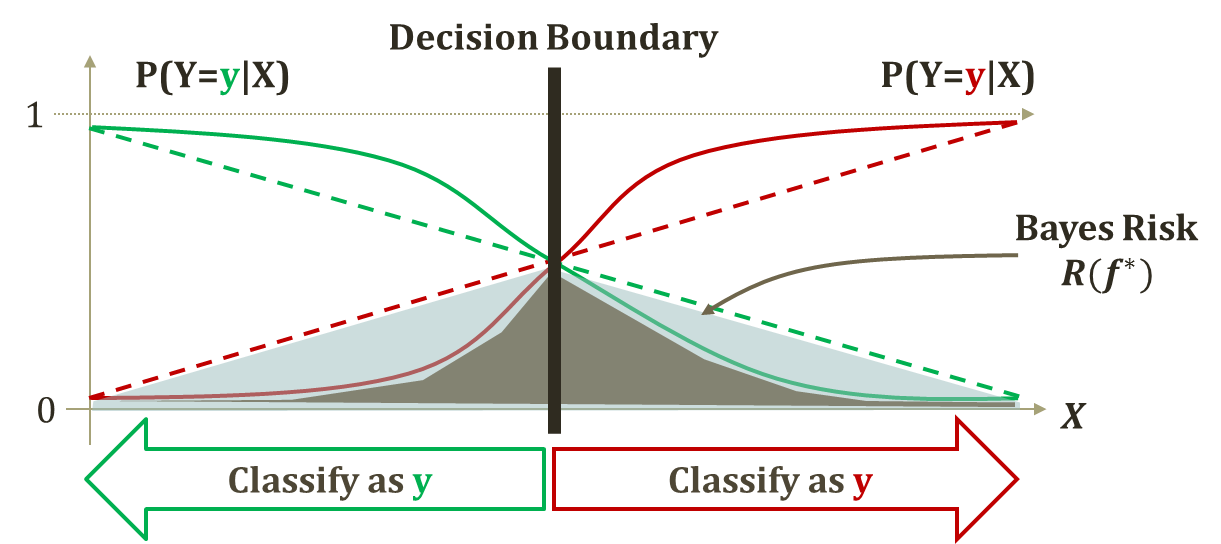
\includegraphics[scale=0.5]{Decision_Boundary1}\caption{결정 경계}\label{Fig:5-1}
\end{figure}
\begin{figure}[ht]\centering
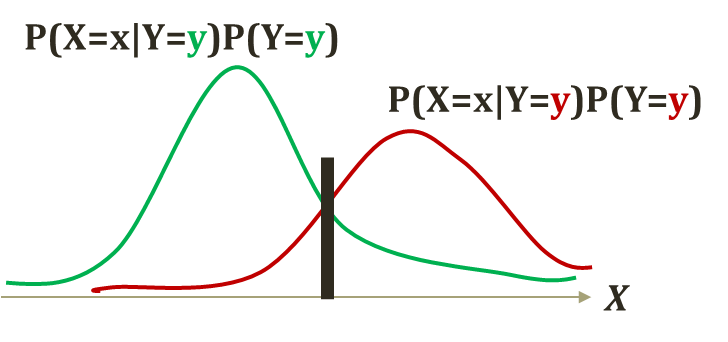
\includegraphics[scale=0.5]{Decision_Boundary2}\caption{조건부 확률의 결정 경계}\label{Fig:5-2}
\end{figure}
\indent 먼저 서포트 벡터 머신(Support vector machine) 자체 설계에 대한 내용을 배워보겠다. 그 전에, 앞서서 다뤘던 확률적인 부분에서 결정 경계(Decision Boundary)를 설정하는 부분을 잠깐 다시 살펴보도록 하겠다. X가 주어진 상황에서 Y가 초록색일 확률과 빨간색일 확률이 그림 1과 같이 변한다고 했을 때, 두 확률이 교차하는 부분에서 결정 경계가 생긴다고 하였다. 그리고 S커브 형태인 Sigmond 함수를 사용하는 이유 중 하나가 바로 결정 경계 근처에서 급격한 확률의 변화를 관측하기 위함이라고 했었다.  
\begin{equation}
\begin{split}
&f^*(x)={argmax}_{Y=y}P(Y=y|X=x)\\
&={argmax}_{Y=y} P(X=x|Y=y)P(Y=y)
\end{split}
\label{eq:5-1}
\end{equation}
\begin{equation}
P(X=x;\mu ,\sigma)=\frac{1}{\sigma\sqrt{2\pi}}e^{-\frac{(x-\mu)^2}{2\sigma^2}}
\label{eq:5-2}
\end{equation}

% 슬라이드 5
\begin{figure}[ht]\centering
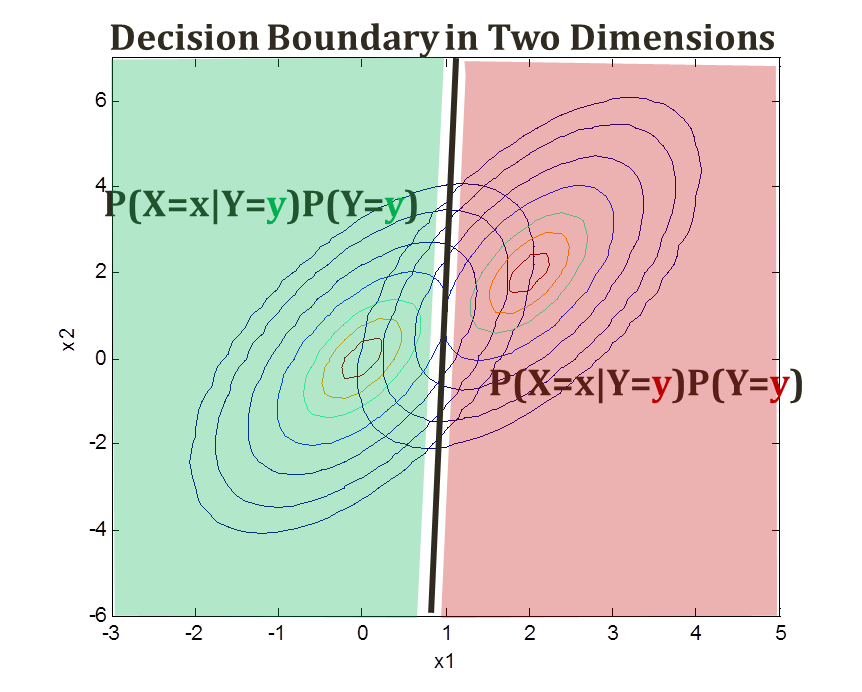
\includegraphics[scale=0.5]{Decision_Boundary3}\caption{2차원의 결정 경계}\label{Fig:5-3}
\end{figure}
\indent 또한 $x_1,x_2$와 같이 2개의 차원을 가지고 있을 경우에도 결정 경계를 가질 수 있다고 했었다. 그림 3에서 보면, 나이브 베이즈 형태로 나타나 있고, 오른쪽 빨간색 영역은 $P(X=x|Y=\textcolor{red}{y})P(Y=\textcolor{red}{y})$의 확률이 더 높고, 왼쪽 초록색 영역은 $P(X=x|Y=\textcolor{green}{y})P(Y=\textcolor{green}{y})$의 확률이 더 높은 영역이다. 아래 수식은 앞서 나왔던 수식으로 X의 특성이 $x_1,x_2$일 때 정규분포에 대한 확률이다.
\begin{equation}
\begin{split}
&P(X=x;\mu ,\sigma)=\frac{1}{\sigma\sqrt{2\pi}}e^{-\frac{(x-\mu)^2}{2\sigma^2}}\\
&\ \ \ \ \ \ \ \ \Downarrow\\
&P(X=(x_1,x_2)|Y=y)=\frac{1}{\sqrt{2\pi}| \sum_y |}exp(-\frac{(x-\mu_y)\sum_{y}^{-1}(x-\mu_y)}{2}
\end{split}
\end{equation}
\\

% 슬라이드 6
\indent 앞서 살펴 봤듯이 결정 경계는 Classification 문제에서 아주 중요한 역할을 한다. 결정 경계가 어떻게 구성이 되었는지에 따라 학습의 유연성이나 성능이 결정이 된다. 앞서 다뤘던 나이브 베이즈나 로지스틱 회귀분석은 모두 확률 기반의 결정 경계를 설정하고 있다. 그런데 아래 그림에서처럼 확률을 배제하고 빨간색 점과 파란색 점이 주어졌을 때의 결정 경계를 정해보라고 하면 어떤 결정 경계가 나은 것일까?\\
\begin{figure}[ht]\centering
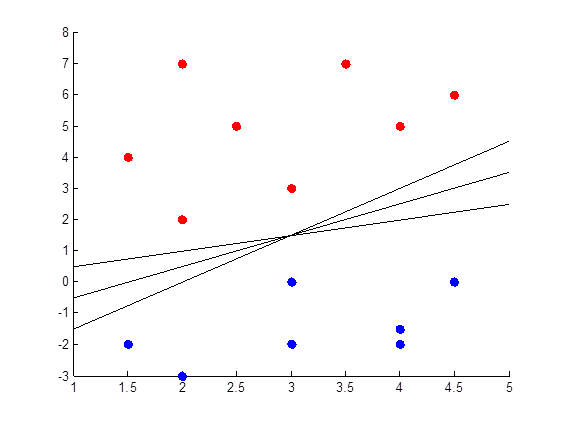
\includegraphics[scale=0.5]{Decision_withoutprob}\caption{확률 배제시 결정 경계}\label{Fig:5-4}
\end{figure}\\
\indent 그림 4에서 결정 경계가 너무 위에 있거나 너무 아래에 있는 경우 빨간색 점을 기계학습 결과로 파란색으로 분류를 할 수도 있고, 파란색 점을 기계학습 결과로 빨간색으로 분류 할 수도 있다. 따라서 결정 경계는 빨간색 점과 파란색 점의 사이에 잡혀져야 한다. 하지만 이 사이에서도 여러 개의 결정 경계가 나올 수 있다. 그 중에서는 선형이 아닌 곡선형태로 잡을 수도 있을 것이다. 하지만 일단은 결정 경계를 선형으로만 잡는다고 가정을 해보자. 역시 다양한 결정 경계가 나올 수 있는데 그림에서는 3개의 결정 경계만을 표현을 해보았다. 그렇지만 이 중에서도 가장 나은 결정 경계가 있을 것이다. \\
\indent 먼저 점과 가까이 있는 결정 경계일수록 안 좋을 수 있다. 그 이유를 생각해보면 먼저 어떤 빨간색 점과 결정 경계가 가까이 있다고 생각해보자. 그리고 후에 이 빨간색 점 주변에 또다른 빨간색 점이 추가가 되었다고 생각을 해보자. 그런데 이 빨간색 점은 결정 경계 아래에 있을 수 있다. 이 경우 학습의 결과 빨간색 점이 파란색으로 분류가 되는 에러가 발생할 수 있다. 그래서 점에서 결정 경계가 멀어질 수록 에러를 줄일 수 있다는 점에서 좋다. 즉, 다른 종류의 점들 사이를 되도록 가운데로 관통하여, 두 클래스로부터 최대한 멀리 떨어져 있는 결정 경계가 좋은 결정 경계가 된다는 뜻이다. \\

% 슬라이드 7
\begin{figure}[ht]\centering
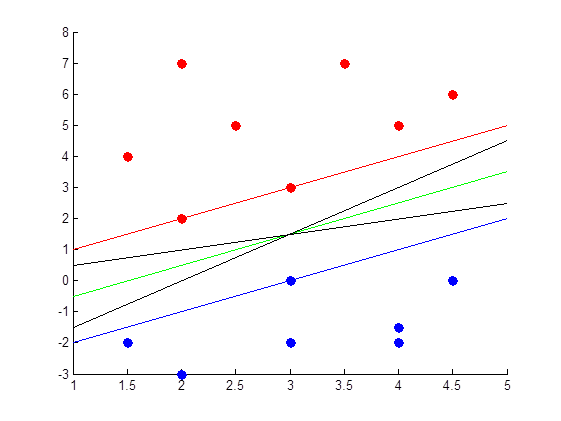
\includegraphics[scale=0.5]{Decision_withmargin}\caption{Margin 활용한 결정 경계}\label{Fig:5-5}
\end{figure}
\indent 그렇다면 어떻게 하면 가운데를 관통하는 결정 경계를 그릴 수 있을까? 다양한 방법이 있을 수 있다. 그 중에 한가지 방법을 살펴보면, 먼저 빨간색 점 가운데 파란색 점들과 가장 가까운 2개의 점을 잇는 직선을 그린다. 위의 그림 5에서는 빨간색 선이 된다. 그리고 이 빨간색 선과 평행한 직선을 내려보며 파란색 점을 만나는 직선을 찾아본다. 위의 그림 5에서는 파란색 선이 된다. 이렇게 될 경우 두 선들 사이에 존재하는 점들은 없게 되고, 두 선들이 빨간색 영역과 파란색 영역의 최전선에 위치한 직선이 된다. 그리고 이 두 직선 사이의 가운데 직선을 찾아본다. 위의 그림 5에서는 연두색 직선이 된다. 이렇게 되면 빨간색 선, 연두색선, 파란색 선들은 평행한 직선들이 된다. 이렇게 선을 찾게 되면 두 영역을 구분하는 직선(빨간색선, 파란색선)간의 거리가 최대화 되고, 가운데 직선은 양쪽 직선까지의 거리가 같게 된다.\\
\indent 이와 같이 되어있는 상황을 어떠한 매커니즘에 의해 만들 수 있다면 결정 경계를 만들 수 있을 것이고, 이 외에 다른 선을 그어 선 사이의 거리를 더 늘릴 수 있는 방법은 없게 된다. 따라서 2 종류의 데이터셋 사이를 관통하면서 가운데를 결정 경계선으로 긋는 방법은 이 방법 밖에 없다는 것이다. 그렇다면 문제점은 무엇이 있을까? 문제점은 바로 직선을 찾을 때 필요한 3개의 점들을 찾는 것이다. 서포트 벡터 머신의 핵심은 이러한 점들을 찾는 것이다. `서포트 벡터 머신'이란 이름이 붙여진 이유를 살펴보면 좀 더 이해하기 쉬울 수 있다. 이렇게 이름이 붙여진 이유는 결정 경계를 서포팅하고 있는 몇개의 점들(벡터형태)을 찾아내는 기계라는 뜻이다. 즉, 결정 경계를 몇개의 벡터들이 서포팅하고 있다고 하여 붙여진 것이다.\\
\indent 이 매커니즘으로 구한 결정 경계선을 나타내는 식은 다음과 같다. 
\begin{equation}
\mathbf{w\cdot x}+b=0
\label{eq:5-4}
\end{equation}
\indent 이 식에서는 총 3개의 파라미터(변수)가 사용되었다. 한 개의 파라미터는 $b$로써 절편을 나타내고, 두 개의 파라미터는 결정 경계선의 수선방향의 벡터 $\mathbf{w}$에 포함되어있다. 그리고 우리는 $x_1,x_2,b$에 대해서 알아보려고 했으므로 변수가 3개이므로 방정식을 풀기 위해서는 3개의 점이 필요하다. 다음으로 Positive case와 Negative case에 대해서 알아보도록 하겠다. 임의로 그림 5에서 파란색 점을 Positive로, 빨간색 점을 Negative로 두고 생각을 해보자. 평면을 식으로 나타낼때 수선벡터와 상수 파트로 나누워진 것처럼 직선도 수선벡터와 상수 파트로 나눌 수 있다. 이 때 파란색 점들이 Positive로 나오기 위해서는 수선 벡터인 $\mathbf{w}$는 파란색점 쪽, 즉 아래방향이 된다. 그리고 연두색 선에 해당하도록 $b$를 정하면 결정 경계식이 연두색 선에 해당하게 된다. 다음으로 두가지 경우를 비교를 해보겠다.
\begin{itemize}\setlength\itemsep{-\parsep}
	\item Positive case인 파란색 점들의 경우 수선벡터방향에 위치하여 있으므로 각 위치 좌표 $\mathbf{x}$를 수식 \eqref{eq:5-4} 에 			대입을 하게 되면 아래과 같은 결과가 나오게 된다.
\end{itemize}
\begin{equation}
\mathbf{w\cdot x}+b>0
\label{eq:5-5}
\end{equation}
\begin{itemize}\setlength\itemsep{-\parsep}
	\item Negative case인 빨간색 점들의 경우 수선벡터방향과 반대방향에 위치하여 있으므로 각 위치 좌표 $\mathbf{x}$ 에 수식 				\eqref{eq:5-4}를 대입을 하게 되면 아래과 같은 결과가 나오게 된다.
\end{itemize}
\begin{equation}
\mathbf{w\cdot x}+b<0
\label{eq:5-6}
\end{equation}
\begin{itemize}\setlength\itemsep{-\parsep}
	\item Confidence level의 경우 약간의 장치를 통해 계산할 수 있다. 바로 $y_j$라는 값을 추가하는 것이다. 이 값은  j번째 점에 대한 값으로, 해당하는 점이 Positive일 경우는 1, Negative일 경우는 -1로 설정을 한다. 그렇게 되면 Confidence level을 뜻하는 아래의 수식은 Positive, Negative 상관없이 항상 양수가 나오게 된다. 그리고 우리는 이 Confidence level을 최대한 높이는 것이 목적이다.
\end{itemize}
\begin{equation}
(\mathbf{w\cdot x_j}+b)y_j
\label{eq:5-7}
\end{equation}\\
\indent 이러한 방법은 Margin을 최대화하는 결정 경계를 찾는 방법인데, 여기서 Margin이란 결정 경계와 가장 가까운 점까지의 수직 거리를 뜻한다. 즉, 연두색 선과 빨간색 선(혹은 파란색 선)까지의 거리를 뜻한다.\\

% 슬라이드 8
\subsection{Margin Distance}
\begin{figure}[ht]\centering
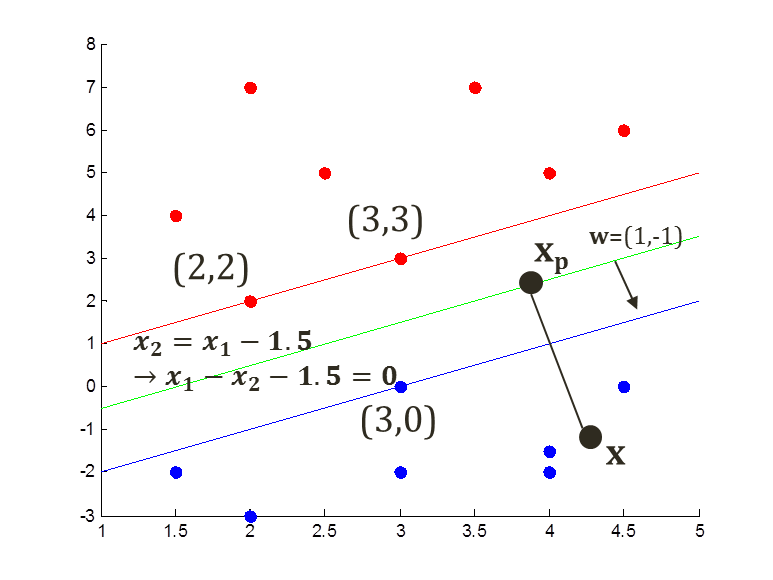
\includegraphics[scale=0.7]{Margin_Distance}\caption{Margin Distance}\label{Fig:5-6}
\end{figure}
\indent 다음으로는 Margin Distance를 계산을 해보도록 하겠다. 먼저 결정 경계식이 다음과 같다고 가정을 하겠다.
\begin{equation}
f(\mathbf{x})=\mathbf{w\cdot x}+b
\label{eq:5-8}
\end{equation}
이 때 점 $\mathbf{x}$가 결정 경계선상에 있다면 $f(\mathbf{x})=\mathbf{w\cdot x}+b=0$이 된다. 그리고 Positive 점에 대해서는 
$f(\mathbf{x})=\mathbf{w\cdot x}+b=a,\ a>0$가 된다. 그림 6에서 살펴보면, $\mathbf{x}_p$의 경우 0의 값을 가지고 $\mathbf{x}$의 경우 양의 값을 가지게 되는 것이다.\\\\
\indent 이제는 이 거리를 식으로 표현을 해보도록 하겠다. 우리가 구하고자 하는 식은 임의의 점 $\mathbf{x}$에서 결정 경계선 까지의 수직거리를 구하고자 하는 것이다. 즉, 점 $\mathbf{x}$에서 결정 경계선에 수선의 발을 내리고, 이 때 수직 거리 선과 결정 경계선이 만나는 점을 $\mathbf{x}_p$로 두었을 때, 점 $\mathbf{x}$와 점 $\mathbf{x}_p$까지의 거리를 구하는 것이다. 여기서 점 $\mathbf{x}$는 점 $\mathbf{x}_p$에서 수선 벡터방향인 $\mathbf{w}$로 $r$의 크기만큼 이동한 것이므로 다음과 같이 나타낼 수 있다. 그리고 여기서 $\mathbf{x}_p$는 결정 경계선상의 점이므로 $f(\mathbf{x}_p)$는 0의 값을 가진다.\\
\begin{equation}
\mathbf{x}=\mathbf{x}_p+r\frac{\mathbf{w}}{\lVert \mathbf{w}\rVert},\ f(\mathbf{x}_p)=0
\label{eq:5-9}
\end{equation}\\
\indent 그리고 수식 \eqref{eq:5-9}의 결과를 $f(\mathbf{x})$에 넣게 되면 다음과 같은 결과를 얻을 수 있다. 여기에서 $r\lVert \mathbf{w}\rVert$가 앞에서 우리가 임의의 양수로 뒀던 $a$가 되는 것이다.\\
\begin{equation}
f(\mathbf{x})=\mathbf{w}\cdot \mathbf{x}+b=\mathbf{w}(\mathbf{x}_p+r\frac{\mathbf{w}}{\lVert \mathbf{w}\rVert})+b=\mathbf{wx}_p+b+r\frac{\mathbf{w}\cdot \mathbf{w}}{\lVert \mathbf{w}\rVert}=r\lVert \mathbf{w}\rVert
\label{eq:5-10}
\end{equation}\\
\indent 최종적으로 Margin Distance $r$은 다음과 같은 결과를 얻게 된다.\\
\begin{equation}
r=\frac{f(\mathbf{x})}{\lVert \mathbf{w}\rVert}
\label{eq:5-11}
\end{equation}

% 슬라이드 9
\subsection{Margin의 최대화}
\begin{figure}[ht]\centering
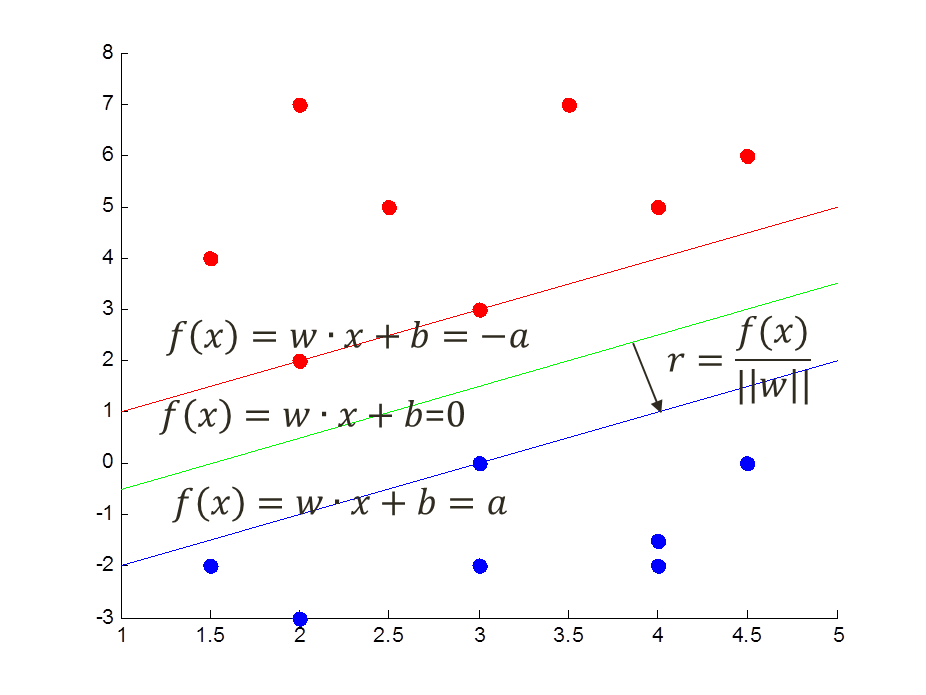
\includegraphics[scale=0.5]{Maximizing_Margin}\caption{Margin의 최대화}\label{Fig:5-7}
\end{figure}
\indent 이렇게 Margin Distance를 구하는 방법에 대해서 알아보았는데, 그렇다면 좋은 결정 경계와 어떤 관계가 있을까? 앞에서 잠깐 언급했듯이 두 종류의 클래스로부터 최대한 멀리 떨어져 있는 것이 좋은 결정 경계가 된다고 하였다. 이말은 즉, Margin을 최대화 한다는 것과 같은 말이다. Margin distance 수식 \eqref{eq:5-11}에서 $f(\mathbf{x})=a$로 바꾸면 $$r=\frac{a}{\lVert \mathbf{w}\rVert}$$로 나타낼 수 있다. 그리고 여기에서 Margin은 빨간색 점까지의 거리와 파란색 점까지의 거리로 2가지 종류가 있다. 우리는 양쪽 사이드(빨간색, 파란색)를 모두 고려를 해야 한다. 따라서 최적의 결정 경계를 찾는 문제는 다음과 같이 표현이 될 수 있다.\\
\begin{equation}
max_{\mathbf{w},b} 2r=\frac{2a}{\lVert \mathbf{w}\rVert}\ \ \ s.t.\ (\mathbf{wx_j}+b)y_j\geq a,\ \forall j
\label{eq:5-12}
\end{equation}\\
이 수식의 목적은 Margin Distance를 최대화하는 $\mathbf{w}$와 $b$를 찾는 것이 목표이다. 따라서 목적 함수가 간단할수록 좋을 것이다. $a$는 임의의 숫자이므로 1로 표준화 시킬 수 있다. 또한 max$\frac{1}{\lVert \mathbf{w}\rVert}$는 min$\lVert \mathbf{w}\rVert$와 같은 함수이므로 수식 \eqref{eq:5-13}은 다음과 같이 변형시킬 수 있다. 이 방법은 maximize 문제를 minimize 문제로 바꾼 것이다.\\
\begin{equation}
min_{\mathbf{w},b} {\lVert \mathbf{w}\rVert}\ \ \ s.t.\ (\mathbf{wx_j}+b)y_j\geq 1,\ \forall j
\label{eq:5-13}
\end{equation}\\
\indent 위의 수식을 보면 이 최적화 문제는 2차 최적화 문제가 된다. 그 이유는 $\mathbf{w}$에는 $w_1,w_2$와 같이 개별 요소가 존재하므로 $\lVert \mathbf{w}\rVert$는 $\sqrt{w_1^2+w_2^2}$와 같은 형태가 나오기 때문이다. 루트 함수는 단조증가함수이기 때문에 $w_1^2+w_2^2$부분을 신경을 써야 하기 때문에 2차 최적화 문제가 된다. 2차 최적화 문제를 풀기 위해서 선형계획법(Linear programming)이 아닌 2차계획법(Quadratic programming)을 사용 하여야 한다. 하지만 이는 최적화 관련 내용으로 간단히 설명할 수 없으므로 이 책에서는 다루지 않을 것이다. 하지만 자주 사용하는 방법론이므로 잘 모른다면 공부를 해보는 것을 추천한다. 이런 최적화 문제를 가장 쉽게 풀 수 있는 것은 R이나 Matlab과 같은 프로그램이다. 이러한 프로그램들에는 최적화 문제를 풀어주는 기능이 있다. 이를 통해 서포트 벡터 머신의 $\mathbf{w}$를 추론할 수 있다.\\

% 슬라이드 10
\subsection{Hard Margin}
\indent 하지만 실제로 선 하나로 두 종류로 깔끔하게 나누는 경우는 드물다. 아래의 그림에서 살펴보면 그림 8은 기존의 데이터셋이고, 그림 9는 새로운 데이터 값이 3개 추가된 경우이다.\\
\begin{figure}[ht]\centering
\parbox[t]{5cm}{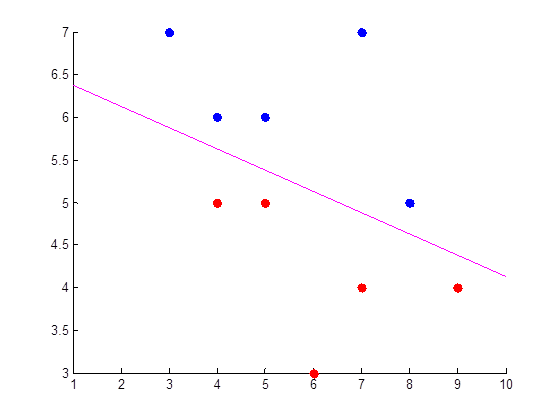
\includegraphics[scale=0.4]{HardMargin1}\caption{기존의 데이터셋}\label{Fig:5-8}}\hspace{0.5cm}
\parbox[t]{5cm}{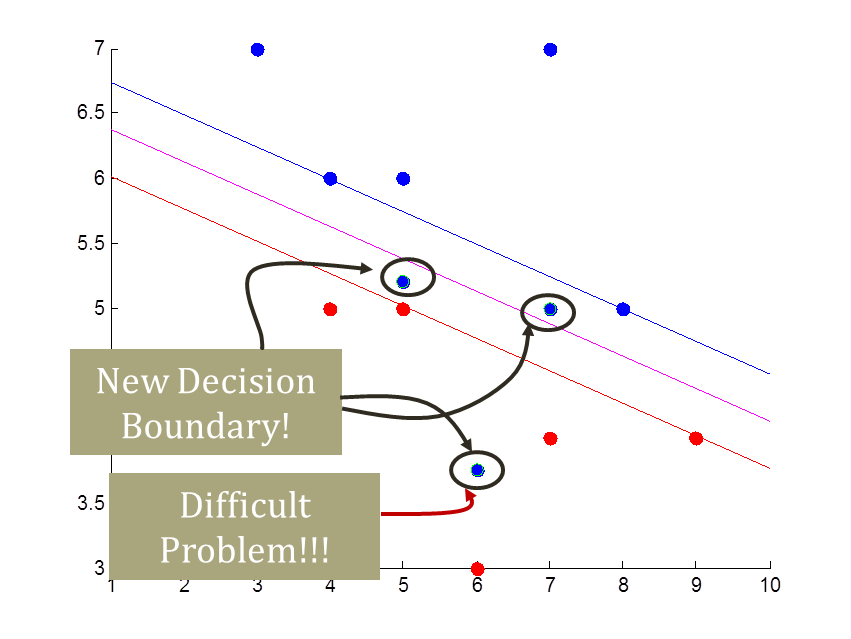
\includegraphics[scale=0.35]{HardMargin2}\caption{추가된 데이터셋}\label{Fig:5-9}}
\end{figure}\\
\indent 그림 8의 경우는 선 한개로 빨간색, 파란색 두 종류의 점을 나눴지만, 그림 9의 경우에 조금 다른 양상을 보인다. 먼저 새로 추가된 파란색 점들은 3개가 있는데 보라색 선 근처의 2개의 점은 새로운 결정 경계(Decision Boundary)를 잡으면 해결이 되지만, 빨간색 점 사이에 위치해 있는 점은 새로운 선을 긋는다고 해서 두 종류의 점들을 완벽하게 나눌 수 없다. 하지만 현실에는 이런 경우가 매우 많다. 서포트 벡터 머신(SVM)은 모든 클래스에 대해서 가장 가까운 훈련 데이터 포인트까지의 거리들이 최대 거리가 되도록 초평면 집합을 만드는 것이다. 그리고 여기에서 어떤 결정 경계 위쪽은 모두 A라는 클래스, 아래쪽은 모두 B라는 클래스에 속하는 경우를 Hard한 결정 경계라고 해서 Hard margin 이라고 한다. Hard margin SVM은 어떠한 에러도 허용하지 않는 것이다.\\
\indent 하지만 현실에서는 에러가 너무 많기 때문에 Hard margin SVM을 쓰기 위해서는 에러를 조금 포함할 수 있도록 만들어야 한다. 그래서 Hard margin SVM을 수정을 해야하는 데, 그 전략은 크게 2가지가 있을 수 있다. 첫번째 전략은 결정 경계는 선형이라고 가정을 하고 에러는 일부 인정을 하고 이 일부는 우리가 정해주는 방법이 있다. 이 방법이 바로 Soft margin SVM이라고 한다. 이렇게 할 경우 결정 경계는 여전히 선형을 유지한 상태에서 에러 케이스를 받아주게 된다. 이를 바로 다음 절에서 배울 것이다. 또 다른 전략은 결정 경계가 선형이 아는 곡선형이라고 두는 것이다. 이렇게 하기 위해서는 Kernel trick이라는 방법이 필요하고 이는 Soft margin을 다룬 뒤에 그 다음 절에서 다룰 것이다.\\

% 슬라이드 11
\section{Soft margin과 페널티}

% 슬라이드 12
\indent 앞선 절에서 서포트 벡터 머신이 무엇인지 서포트 벡터 머신의 설계에 대해서 다뤘었다. 그리고 결정 경계를 서포트 하는 벡터(점)들을 찾아내어 최적화 문제를 풀어내기 때문에 서포트 벡터 머신이라고 이름이 붙어졌다고 이야기 했었다. 이 때 Hard margin SVM 같은 경우에는 여러 에러 상황에 대해서 대처가 안된다고 하였다. 이번 절에서는 이를 해결하기 위한 첫번째 전략인 Soft margin SVM과 Penalization에 대해서 배워보도록 하겠다.\\
\begin{figure}[ht]\centering
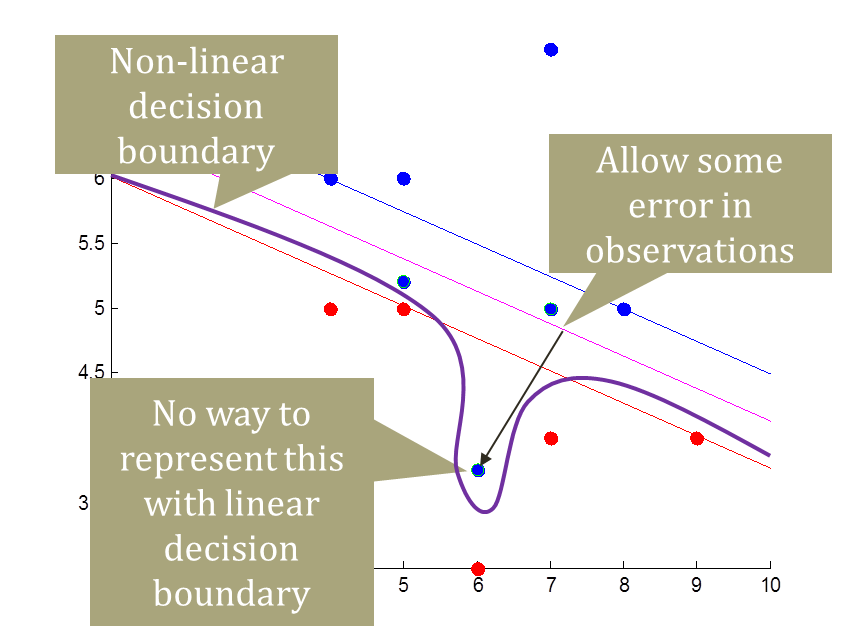
\includegraphics[scale=0.5]{ErrorCase}\caption{SVM에서 에러 사례}\label{Fig:5-10}
\end{figure}\\
\indent 앞선 절 마지막에서 다뤘던 내용을 생각을 해보자. 실제 사례들을 다룰 때에는 결정 경계로 분류할 때 에러가 발생할 수 있다고 하였다. 그리고 이에 대한 해결책으로 2가지를 제안을 했었다. 첫번째 방법은 결정 경계를 복잡하게 비선형으로 만들어 모든 점들을 맞게 분류를 하는 방법이었다. 그리고 다른 방법은 몇 개의 에러에 대해서 인정을 하고 허용하는 방법이 있었다. 그리고 에러의 경우에 대해서는 거리만큼 Penalization(벌칙)을 줄 수도 있다. 이 절에서는 두번째 방법에 대해서 다루도록 하겠다.\\

% 슬라이드 13
\begin{figure}[ht]\centering
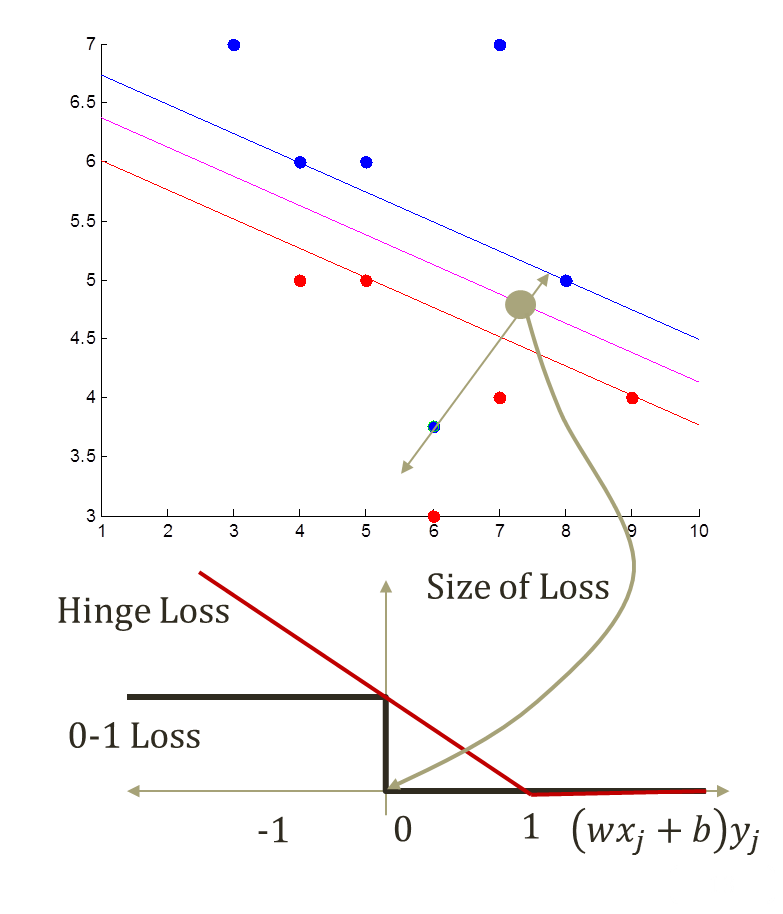
\includegraphics[scale=0.5]{ErrorHandling}\caption{SVM에서 에러 처리}\label{Fig:5-11}
\end{figure}
\indent 그렇다면 에러는 어떻게 다뤄야 할까? 이 방법에 대해서 알아보도록 하겠다. 그림 11에서 보면 빨간색 점들 사이에 파란색 점 하나가 존재한다. 이 경우에는 선형 결정 경계로는 정확하게 분류가 되지 않는다. 우선 결정 경계가 어떻게 만들어 졌는지를 생각해보자. 결정 경계는 수식 \eqref{eq:5-13}에서 2차계획법을 통해 법선 벡터 ${\lVert \mathbf{w}\rVert}$ 구하여 만들어졌다. 우리는 수식 \eqref{eq:5-13}의 목적 함수에서 에러와 관련된 요소를 추가하여 에러를 처리하고자 한다. 이렇게 에러를 처리하는 방법에는 2가지 방법이 있다. 이 때 에러에 관한 페널티 점수를 부여하는 방법은 Loss 함수와 관련이 있다. 그림 11의 아래 함수를 참고하여 설명을 하겠다. `0-1 Loss' 함수는 기준점(결정 경계)로 부터 양의 방향에 있을 때는 0의 값을 갖고 음의 방향에 있을 때는 1의 값을 가지는 함수이다. 그리고 `Hinge Loss' 함수는 기준점(결정 경계)로 부터 양의 방향으로 한계선(파란색 선) 이상일 때는 1의 값을 가지고 그 선을 넘어가는 순간부터 음의 방향으로 갈 때 값이 점차 커지는 함수이다. \\
\indent 첫번째 방법은 에러가 발생한 횟수만큼 페널티를 주는 것으로 `0-1 Loss' 함수를 활용한 방법이다. 하지만 이 방법의 경우에는 결정 경계로부터 거리와 상관 없이 에러라면 똑같은 페널티가 부여된다는 문제점이 있다. 이 방법에 맞춰 수식을 바꿔보면 다음과 같다. C는 절충 매개변수이고 $\#_{error}$는 에러 발생한 수이다. 
\begin{equation}
\begin{split}
&min_{w,b} {\lVert w\rVert}+C\times \#_{error}\\
&s.t\ \ (wx_j+b)y_j\geq 1, \forall j
\end{split}
\label{eq:5-14}
\end{equation}
\indent 두번째 방법은 에러가 발생한 거리에 따라 페널티를 다르게 주는 것으로 `Hinge Loss' 함수를 활용한 방법이다. 여기서 slack variable(여유 변수)를 도입을 하는데, 활용 방법은 분류가 잘못 되었을 때 slack variable $\xi_j>1$로 두는 것이다. 이에 따라 수식 \eqref{eq:5-13}을 바꿔보면 다음과 같다. 
\begin{equation}
\begin{split}
&min_{w,b} {\lVert w\rVert}+C\Sigma_{j} \xi_j\\
&s.t.\ \ (wx_j+b)y_j\geq 1-\xi_j, \forall j\\
&\ \ \ \ \ \ \ \xi_j\geq 0,\ \forall j
\end{split}
\label{eq:5-15}
\end{equation}
\indent 수식을 살펴보면 먼저 C라는 매개변수는 slack variable에 대해서 목적 함수에 어느 정도로 영향을 줄지에 대한 강도를 조절하는 절충 매개변수이다. 그리고 목적함수는 기존 목적함수에서 slack variable로 생긴 요소($C\Sigma_{j} \xi_j$)까지 더한 함수를 최소화하는 변수를 찾게 된다. 다음으로 조건식도 조금 바뀌게 된다. 첫번째 조건식에서 우변이 1에서 $1-\xi_j$로 바뀌었는데, 그 이유는 일부 j에 대해서는 에러를 허용하기 위해서이다. 그리고 두번째 조건식은 slack variable이 0보다 크다는 조건이다. 하지만 이렇게 최적화 식을 바꾸었을 때는 C라는 새로운 매개변수를 정해줘야하는 문제가 발생한게 된다.

% 슬라이드 14
\subsection{Soft margin SVM}
\indent 이처럼 slack variable을 써서 결정 경계를 정하는 모델을 Soft margin SVM(서포트 벡터 머신)이라고 할 것이다. 아래 그림 12에서 보면 빨간색 글씨로 표시한 3개의 점은 slack variable이 0보다 크고 나머지 점들은 0의 값을 가지게 된다.\\
\begin{figure}[ht]\centering
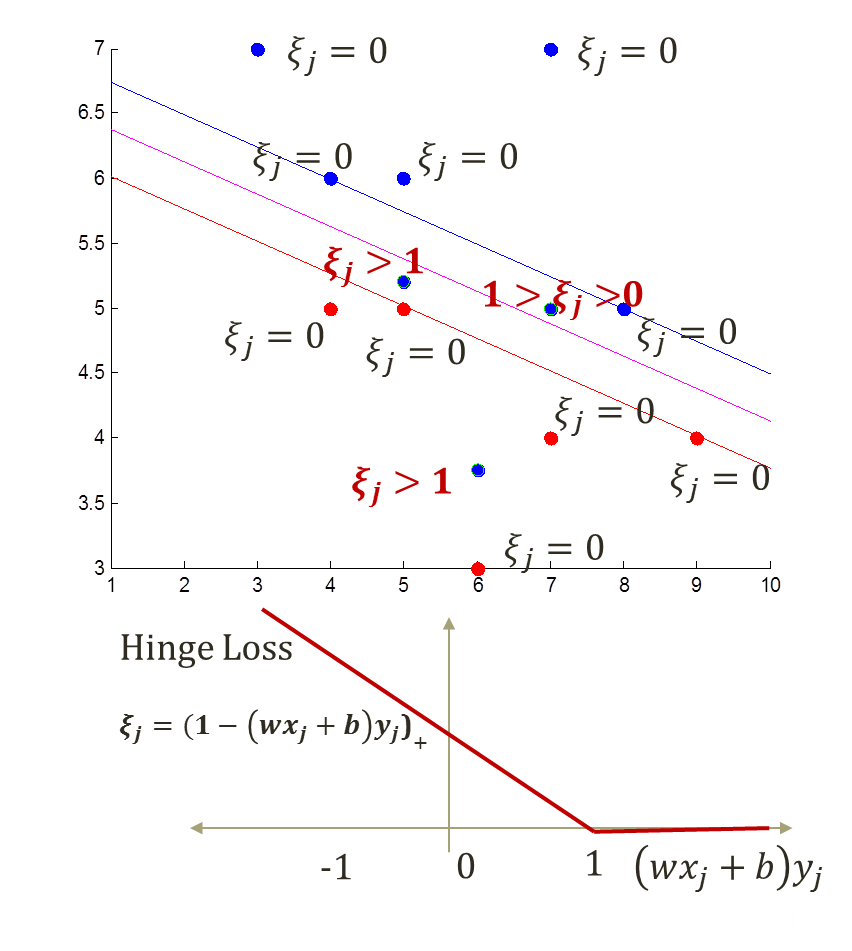
\includegraphics[scale=0.5]{SoftMargin}\caption{Soft margin SVM}\label{Fig:5-12}
\end{figure}\\
\indent Hard margin SVM에서는 어떠한 포인트가 자신의 영역에서 결정 경계를 넘는 순간 infeasible한 문제가 되어서 새로운 결정 경계를 구할 수 없게 되었지만 Soft margin SVM으로 만들게 되면 결정 경계를 항상 생성할 수 있게 된다. 즉, 조건식에 slack variable을 추가하여 부드럽게(soft하게) 만드는 것이다. 대신에 잘못 분류한 것에 대해서는 페널티를 주어, 자동으로 에러를 고려하도록 모델링을 한 것이다.

% 슬라이드 15
\subsection{Loss 함수}
\indent 여기서 잠시 로지스틱 회귀분석과 Loss 함수 관점에서 비교를 해보도록 하겠다. \\
\begin{figure}[ht]\centering
\parbox[t]{5cm}{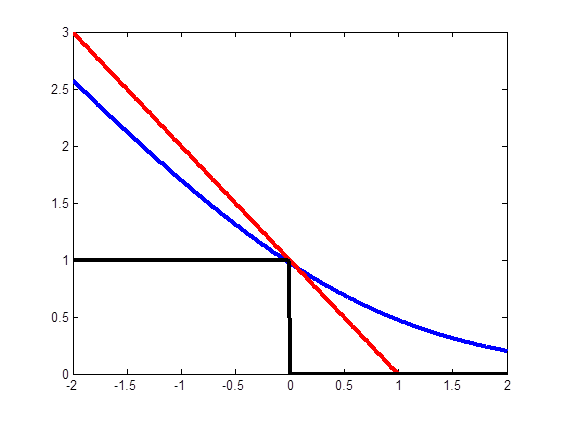
\includegraphics[scale=0.5]{Lossfunction}\caption{Loss 함수}\label{Fig:5-13}}\hspace{1cm}
\parbox[t]{5cm}{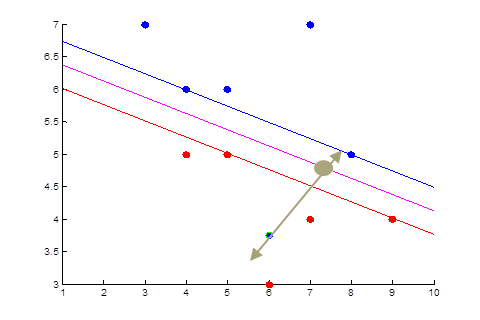
\includegraphics[scale=0.5]{Lossfunction2}\caption{결정 경계와 Loss}\label{Fig:5-14}}
\end{figure}\\
\indent Loss 함수는 $\xi_j=loss(f(x_j),y_j)$로써 함수값 $f(x_j)$와 실제값 $y_j$간의 차이를 의미한다. 그림 13에서 보면 검은색 선이 `0-1 Loss 함수', 빨간색 선이 `Hinge Loss 함수'이다. Hinge Loss 함수는 다음과 같은 식을 가지는데
\begin{equation}
\xi_j=(1-(wx_j+b)y_j)_{+}
\label{eq:5-16}
\end{equation}
Hinge는 경첩이란 뜻인데 빨간색 선이 검은색 선 귀퉁이에 걸려있는 것이 문을 열었을 때 걸리는 것과 같다고 해서 붙어진 이름이다. 한편 로지스틱 회귀분석에서도 Loss 함수가 있다. 바로 `Log loss' 함수이다. 기존의 로지스틱 회귀분석식은 아래와 같이 바꿀 수 있다.
\begin{equation}
\begin{split}
\hat{\theta}&={argmax}_{\theta}\Sigma_{1\leq i\leq N} \log(P(Y_i|X_i;\theta))\\
&={argmax}_{\theta} \sum_{1\leq i\leq N}\{Y_i X_i \theta - \log(1+e^{X_i \theta})\}
\end{split}
\end{equation}
\indent 여기서 마지막 식 $- \log(1+e^{X_i \theta})$을 살펴보면 Hinge loss 함수의 뒷 부분인 $-(wx_j+b)y_j$과 유사하다. 그래서 이 함수를 그래프로 그려보면 그림 13에서 파란색 선에 해당하게 된다. 그리고 Log loss 함수는 다음과 같이 표현된다.
\begin{equation}
\xi_j=-\log(P(Y_j|X_j,w,b))=\log(1+e^{(wx_j+b)y_j})
\label{eq:5-17}
\end{equation}
\indent 그렇다면 어떤 Loss 함수가 선호될까? 답은 상황에 따라서 다르다는 것이다. SVM이 더 최근에 만들어졌다고 해서 Hinge Loss 함수가 무작정 더 좋다고 얘기할 수 없다. SVM 같은 경우에는 양쪽으로 완전히 갈릴 수 있다는 관점에서 본 경우이다. 예를 들어 Hinge loss 함수의 경우에는 특정점 이상에서는 Loss 함수값이 0이다. 하지만 Log loss 함수의 경우에는 항상 Loss 함수값을 가지고 있다. 즉, Log loss 함수의 경우에는 안전한 구역에 있다고 하더라도 페널티를 주는 것이다. 그리고 경계선(Front Line)을 넘어서도 급격히 변하기 보다는 유연하게 변하는 것이다. 그래서 어떤 머신러닝 테크닉을 사용하느냐에 따라서 Loss 함수가 달라지기 때문에 문제에 맞춰 알고리즘을 선택하여야 한다.\\

% 슬라이드 16
\subsection{Loss 함수의 강도}
\indent 그리고 앞서서 수식 \eqref{eq:5-15}에서 Hinge loss 함수를 사용하면 최적화의 목적함수에 C라는 절충 매개변수가 추가 된다고 하였다. 그리고 이 값을 정해주어야 하는 문제점이 있다고 했었다. 그렇다면 C 값을 어떻게 두는 것이 좋을까? 다음은 그림들은 C 값을 달리주면서 얻어낸 실험 결과 데이터들이다.\\
\begin{figure}[ht]\centering
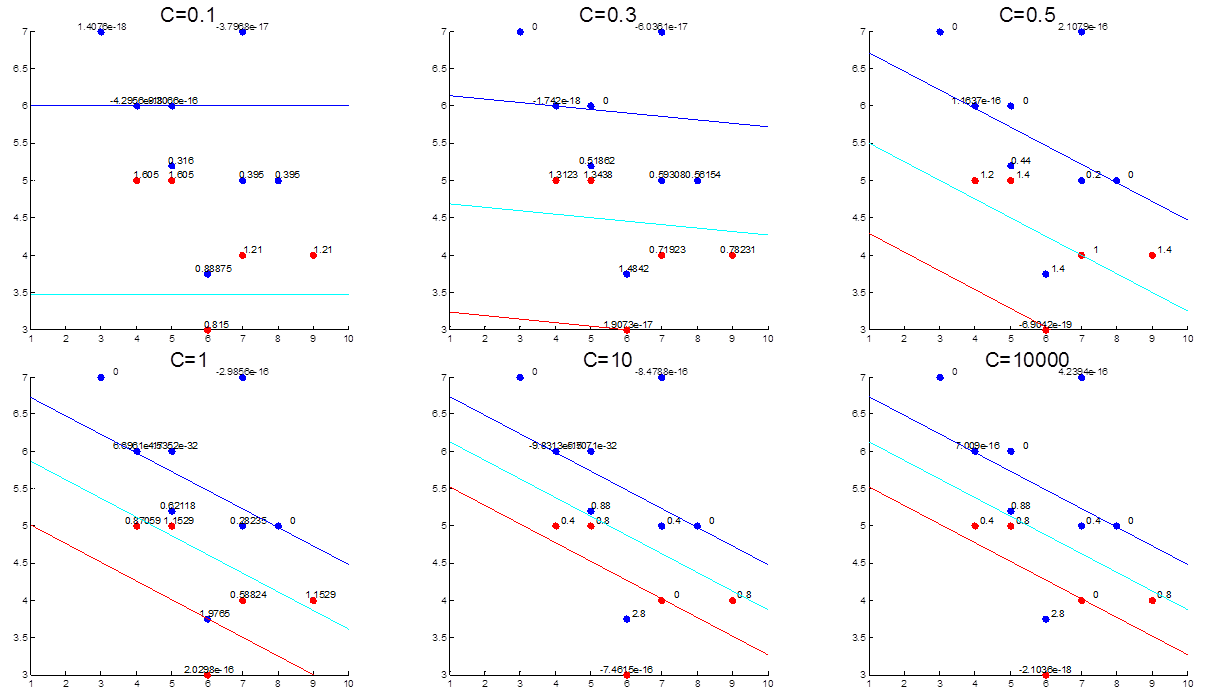
\includegraphics[scale=0.5]{Strength_loss}\caption{C 값에 따른 결과 데이터}\label{Fig:5-15}
\end{figure}\\
\indent 위 그림 15에서 보면 C 값을 0.1 부터 10000까지 다양하게 바꿔보았다. 그 결과를 봐보면 C 값이 작을 때는 결정 경계가 잘 생성이 되지 않았다. 그림에서 하늘색 선이 결정 경계선인데 C=0.1 일 때는 결정 경계선이 빨간색 점과 파란색 점 아래에 생겼다. 이 결과가 의미하는 것은 C 값이 매우 작다 보니 penalization(벌칙)이 매우 적게 적용 되버린 것이다. 즉, 결정 경계를 넘어가도 크게 페널티가 없어 에러가 영향력이 작게 되어버린 것이다.\\
\indent  그리고 C 값을 점차 늘려가다보니 C=1 정도가 됬을 때 어느 정도 결정 경계의 형태를 갖춘 결과가 나왔다. 그리고 C 값이 10 이상이 되면 결정 경계의 형태가 고정이 되는 양상을 보인다. 그 이유는 C 값이 어느 정도 큰 값이 되면 이 페널티의 영향력이 충분히 커서 C 값을 더 키워도 결졍 경계의 형태의 변화에 별 다른 차이가 없게 되는 것이다. 그래서 C를 무조껀 크게 잡아도 상관이 없다는 주장을 하는 사람들이 있다. 하지만 우리가 가진 데이터의 대한 확신이 어느 정도 있느냐에 따라서 C 값을 정해야 할 것이다. 우리가 가지고 있는 데이터셋이 아닌 미래에 들어올 데이터는 전혀 다른 형태를 띌 수도 있기 때문이다.\\
\indent 이 절에서는 soft margin SVM을 만들고 이 과정에서 쓰이는 C라는 매개변수가 어떤 특성을 보이는 지에 대해 알아보았다. 또한 penalization에서 써였던 Loss 함수에 대해서도 알아보았다. 다음 절에서는 선형 결정 경계가 아닌 비선형 결경 경계를 만드는 방법에 대해서 다뤄보도록 하겠다.\\


% 슬라이드 17
\section{Kernel trick}
\indent 이번 절에서는 kernel trick을 이용하여 선형이 아닌 비선형의 결정 경계를 가진 서포트 벡터 머신을 만드는 방법에 대해서 알아보도록 하겠다.\\

% 슬라이드 18
\subsection{SVM 재검토}
\begin{figure}[ht]\centering
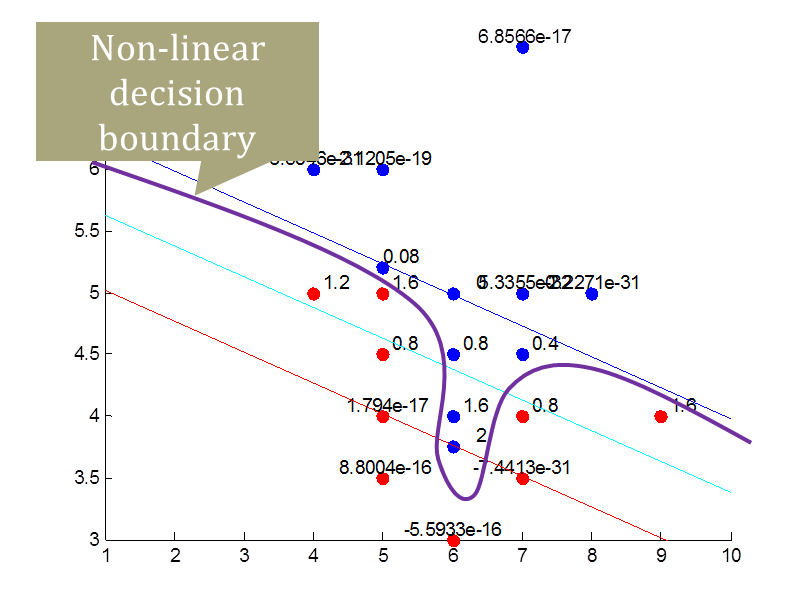
\includegraphics[scale=0.5]{ErrorSVM}\caption{비선형 결정 경계가 필요한 경우}\label{Fig:5-16}
\end{figure}
\indent 먼저 위와 같은 데이터셋이 주어졌다고 생각을 해보자. 그림 16의 파란점들을 보면, 단순히 한 개의 파란색 점이 동떨어져 있는 것이 아니고 여러 개의 파란색 점이 튀어나오는 듯한 트렌드를 가진 것을 확인 할 수 있다. 이 경우에 선형 결정 경계를 하나 정하고 몇 개의 파란점들은 에러 처리를 하는 것이 과연 옳은 것일까? 당연히 아닐 것이다. 이 데이터의 경우에는 보라색 선과 같이 비선형의 결정 경계를 가질 거라는 것이 자명하다. 그래서 데이터를 잘 표현하기 위해서는 결정 경계를 이와 같이 비선형으로 만들어주는 과정이 필요할 것이다. 따라서 이번 절에서는 모델을 좀 더 복잡하게 만들어 비선형의 결정 경계를 만드는 방법에 대해서 배워보도록 하겠다. 그 전에 잠깐 언급해야할 내용이 있는데, 우리가 모델을 복잡하게 만든다는 것은 우리가 가진 데이터가 복잡하기 때문에 필요한 과정이다. 따라서 우리가 가진 데이터가 복잡하지 않다면 굳이 모델을 복잡하게 만들 필요가 없을 것이다. 즉, 모델을 복잡하게 만들기 전 가지고 있는 데이터의 특성을 먼저 잘 알아보는 것이 중요하다.\\

% 슬라이드 19
\begin{figure}[ht]\centering
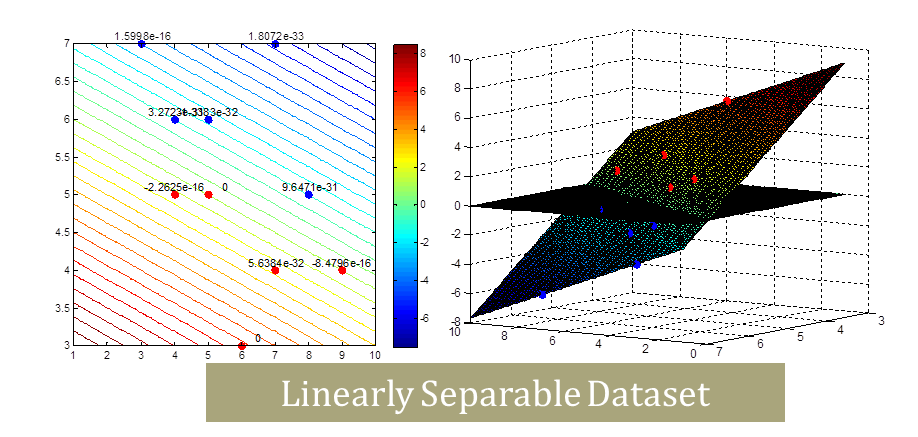
\includegraphics[scale=0.7]{Linear_Dataset}\caption{선형으로 분류 가능한 데이터셋}\label{Fig:5-17}
\end{figure}
\indent 그림 17은 선형 결정 경계로 분류 가능한 데이터셋으로 나타내본 결정 경계의 형태이다. 왼쪽 그림은 연두색 선을 기준으로 위쪽은 파란점들이 있고 아래쪽은 빨간점들이 있는 것을 확인할 수 있다. 그리고 결정 경계 식에서 상수 값에 따라 결정 경계의 위치가 달라지게 되고 왼쪽 그림에서 보면 선의 색깔로 그 차이를 표현을 해보았다. 오른쪽 그림은 평면으로 나타내본 결과로써 3차원에서 선형(평면) 결정 경계로 파란점과 빨간점을 분류한것을 확인 할 수 있다.\\
\begin{figure}[ht]\centering
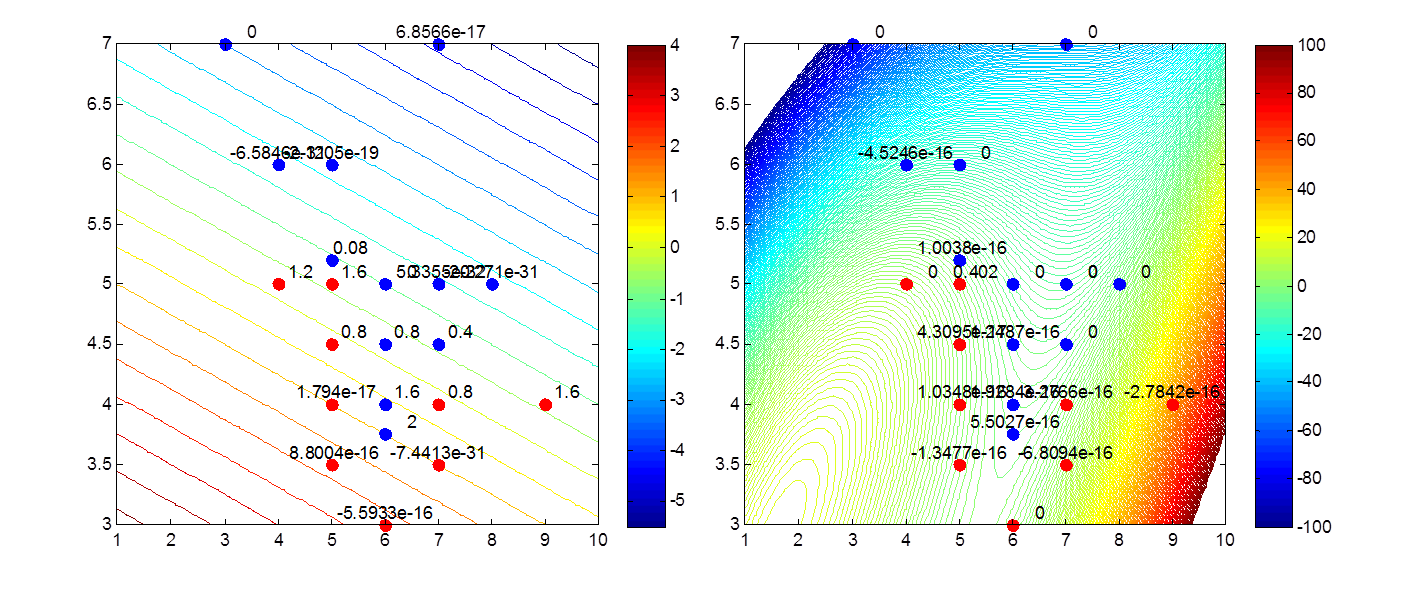
\includegraphics[scale=0.5]{Linear_Decisionboundary}\caption{선형으로 분류 불가능한 데이터셋}\label{Fig:5-18}
\end{figure}\\
\indent 그림 18은 데이터셋이 선형으로 구분이 잘 되지 않는 경우를 나타낸 것이다. 왼쪽 그림은 선형 결정 경계들을 나타낸 그림으로 연두색 선이 결정 경계선으로 soft margin SVM으로 에러를 허용한 경우가 된다. 하지만 이 결정 경계선은 데이터가 가진 특성을 잘 반영하지 못했다. 오른쪽의 그림을 보면 마찬가지로 연두색 선이 결정 경계가 된다. 하지만 왼쪽 그림과는 다르게 연두색 선을 연결을 하면 비선형으로 데이터가 가진 특성에 맞춰서 나타난다는 것을 확인할 수 있다. 이렇게 비선형으로 만드는 방법은 우리가 전에 선형 회귀분석에서 각 항들을 곱하여 차원을 높였던 테크닉과 유사하게 할 수 있다. 예를 들어 $x_1,x_2$로 2차원의 데이터에 대해서 SVM에 쓰일 차원을 다음과 같이 높일 수 있다는 것이다.
\begin{equation}
\varphi(<x_1,x_2>)=<x_1,x_2,{x_1}^2,{x_2}^2,x_1x_2,{x_1}^3,{x_2}^3,{x_1}^2 x_2,x_1{x_2}^2>
\label{eq:5-18}
\end{equation}
\indent 이와 같이 차원을 높여 SVM을 돌린 결과가 그림 18에서 오른쪽 그림에 해당한다. 우리는 앞선 수식 \eqref{eq:5-18}처럼 차원을 확장시킬 수 있지만, 좀 더 똑똑하게 차원을 확장해보는 방법에 대해서 알아보고자 한다. 뿐만 아니라 위의 수식은 최대 3차까지 높여보았는데, 이를 더 크게 무한대차수까지 높이기 위한 방법을 알기 위해 kernel trick에 대해서 배워보도록 하겠다.

% 슬라이드 20
\indent Kernel trick을 제대로 이해하기 위해서는 최적화 문제(Optimization)에 대한 이해가 뒷받침이 되어야한다. 하지만 이 내용을 다루기에는 너무 양이 많고 또 하나의 분야이기 때문에 깊게 다루기에는 무리가 있다. 따라서 이 절의 내용을 제대로 이해하기 위해서는 최적화 이론에 대해서 공부를 하는 것이 더 좋을 것이다. 간략히 얘기를 하지만 기존 최적화 문제가 Primal 문제라고 한다면, 이 문제에 대한 Dual 문제를 정의하여 Dual 문제를 품으로써 기존 최적화 문제의 답을 얻어내는 것이다. 우리가 kernel을 도입하기 위해서는 SVM의 Primal 문제를 Dual 문제로 바꿔야 한다. 여기서 SVM의 Primal 문제라고 하는 것은 우리가 앞서서 계속 다뤘던 최적화 문제와 조건식을 말하고 soft margin SVM에서의 Primal 문제는 다음과 같이 나왔었다.
\begin{equation}
\begin{split}
&min_{w,b} {\lVert w\rVert}+C\Sigma_{j} \xi_j\\
&s.t.\ \ (wx_j+b)y_j\geq 1-\xi_j, \forall j\\
&\ \ \ \ \ \ \ \xi_j\geq 0,\ \forall j
\end{split}
\label{eq:5-20}
\end{equation}
\indent 즉 위와 같은 Primal 문제는 Dual 문제로 바꿔야한다. 이 과정은 머신러닝에 종종 쓰이지만 단지 활용하는 과정이기도 하고 이와 관련된 최적화 분야가 따로 있기 때문에 본 책에서는 간략히 다루도록 하겠다.\\
\indent 결국 SVM은 제한된 2차 계획법(quadratic programming)을 통해 매개변수를 추론하는 것이고 그 형식은 표현하자면 다음과 같다.
\begin{equation}
\begin{split}
&min_{x} f(x)\\
&s.t.\ g(x)\leq 0,\ h(x)=0
\end{split}
\label{eq:5-21}
\end{equation}
\indent SVM에서 Primal 문제를 Dual 문제로 잘 바꾸기 위해서는 Lagrange(라그랑주) method를 알아야 한다. 먼저 Lagrange Prime Function을 다음과 같이 정의를 하면 조건식에 있는 $g(x),h(x)$를 목적 함수에 포함을 시킬 수 있다.
\begin{itemize}\setlength\itemsep{-\parsep}
	\item Lagrange Prime Function:
	\begin{equation}
	L(x,\alpha,\beta)=f(x)+\alpha g(x)+\beta h(x)
	\label{eq:5-22}
	\end{equation}
\end{itemize}
그리고 여기서 $g(x),h(x)$의 앞에는 $\alpha,\beta$라는 Lagrange Multiplier를 붙이게 된다. 그리고 이는 Primal 함수의 조건식에 따라서 변수의 범위가 결정이 된다.
\begin{itemize}\setlength\itemsep{-\parsep}
	\item Lagrange Multiplier:
	\begin{equation}
	\alpha\geq 0,\ \beta
	\label{eq:5-23}
	\end{equation}
\end{itemize}
이를 바탕으로 Dual 문제를 구해보면 Lagrange Dual Function은 다음과 같이 정의가 된다. 여기서 inf 함수는 infimum으로 "최대 하한선"을 말한다. 예를 들어 inf\{1,2.3\}=1 이 된다.
\begin{itemize}\setlength\itemsep{-\parsep}
	\item Lagrange Dual Function:
	\begin{equation}
	d(\alpha,\beta)=inf_{x\in X} L(x,\alpha,\beta)=min_x L(x,\alpha,\beta)
	\label{eq:5-24}
	\end{equation}
\end{itemize}
즉, Lagrange Primal Function의 최소값이 Lagrance Dual Function의 값이 되는 것이다. 또한 Lagrance Prime Function 다음과 같은 성질이 있다.
\begin{equation}
max_{\alpha\geq0,\beta}L(x,\alpha,\beta)=
\begin{cases}
f(x):&\mbox{if }x\mbox{ is feasible}\\
\infty:&\mbox{otherwise}
\end{cases}
\label{eq:5-25}
\end{equation}
따라서 목적 함수 $min_x f(x)$는 다음과 같이 바뀔 수 있다.
$$min_x f(x)\rightarrow min_x max_{\alpha\leq 0,\beta} L(x,\alpha,\beta)$$\\

% 슬라이드 21
\subsection{Primal 과 Dual 문제}
\indent 여기서 Primal 과 Dual 문제를 좀 더 살펴보도록 하겠다. 결국 Primal 문제와 Lagrange Dual 문제는 다음과 같이 표현될 수 있다.\\
\begin{figure}[ht]\centering
\parbox[t]{4cm}{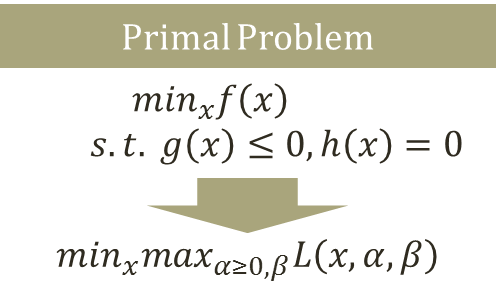
\includegraphics[scale=0.5]{Primal}\caption{Primal 문제}\label{Fig:5-19}}\hspace{2cm}
\parbox[t]{4.5cm}{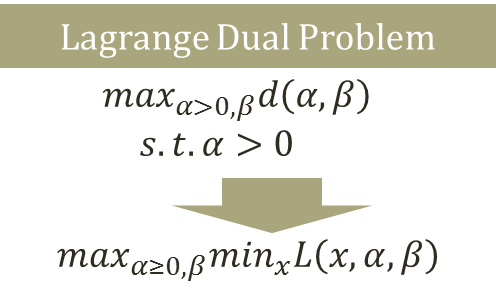
\includegraphics[scale=0.5]{Dual}\caption{Lagrange Dual 문제}\label{Fig:5-20}}
\end{figure}\\
그리고 Primal과 Dual간에는 Weak duality theorem이 성립을 하는데, 이에 대한 자세한 내용은 따로 공부하기를 추천하고 여기에서는 수식만 적고 넘어가도록 하겠다. 여기에서 중요한 점은 Dual 함수의 최대값이 $f(x^*)$의 하한선이라는 것이다.
\begin{itemize}\setlength\itemsep{-\parsep}
	\item Weak duality theorem:\\
	$d(\alpha,\beta)\leq f(x^*)\ for\ \forall\alpha,\forall\beta$\\
	$d^*=max_{\alpha\geq 0, \beta}min_{x} L(x,\alpha,\beta)\leq min_x max_{\alpha\geq 0, \beta} L(x,\alpha,\beta)=p^*$\\
	$Duality\ gap=f(x^*)-d(\alpha^*,\beta^*)$\\
\end{itemize}
그리고 여기에서 Karush-Kunh-Tucker(KKT) 조건이 만족을 하게 되면 Strong duality가 성립을 하게 되고, 다음과 같이 수식이 바뀌게 된다.
\begin{equation}
d^*=max_{\alpha\geq 0, \beta}min_{x} L(x,\alpha,\beta)= min_x max_{\alpha\geq 0, \beta} L(x,\alpha,\beta)=p^*
\label{eq:5-26}
\end{equation}
이 수식이 의미하는 것은 Dual 함수에서 나온 해와 Primal 함수에서 나온 해가 같아지는 상황이라는 것이다. 즉, 지금까지는 Primal 함수를 만들어서 문제를 풀어 왔는데 이제는 Dual 함수로 만들어서 문제를 풀겠다는 것이다. 이를 위해서 KKT 조건이 필요하다고 하였으므로 이에 대해서 알아보도록 하겠다. KKT 조건은 다음과 같다.

% 슬라이드 22
\begin{itemize}\setlength\itemsep{-\parsep}
	\item $\nabla L(x^*,\alpha^*,\beta^*)=0$
	\item $\alpha^*\geq 0$
	\item $g(x^*)\leq 0$
	\item $h(x^*)=0$
	\item $\alpha^*g(x^*)=0$
\end{itemize}
\indent 그리고 KKT 조건과 Strong Duality 간의 관계는 그림 21과 같다.
\begin{figure}[ht]\centering
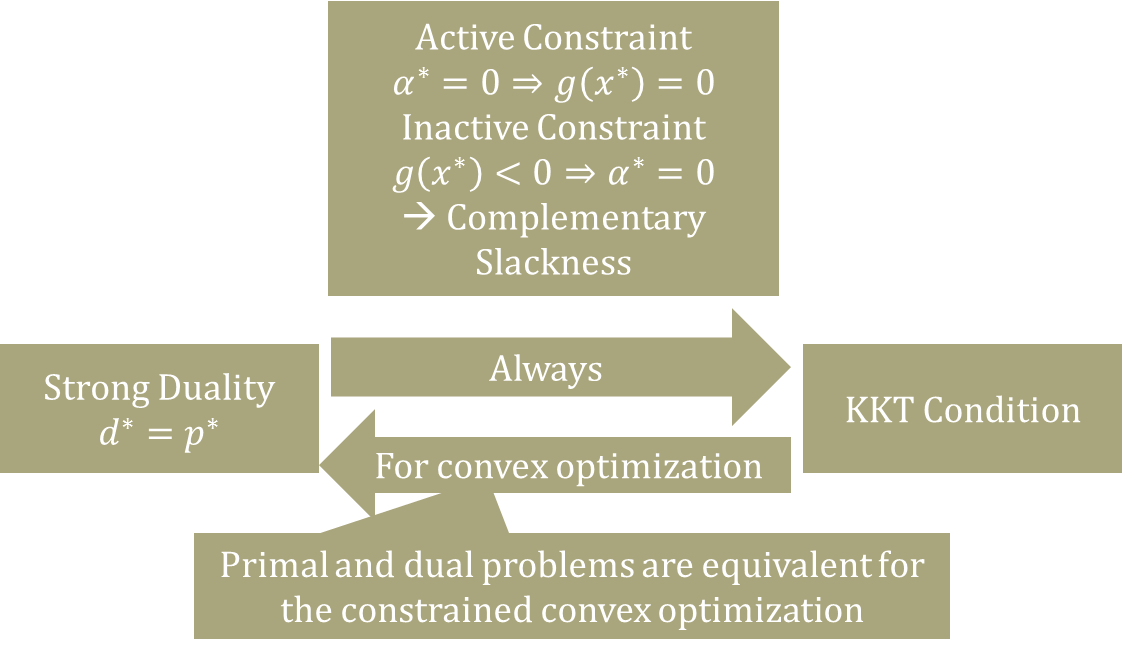
\includegraphics[scale=0.5]{KKT}\caption{KKT 조건과 Strong Duality}\label{Fig:5-21}
\end{figure}


% 슬라이드 23
\subsection{SVM의 Dual}
\indent 이제 앞에서 다뤘던 Primal과 Dual 간의 관계, Lagrange method를 이용하여 SVM의 Dual 함수를 구해보도록 하겠다. 먼저 Lagrange method를 적용하기전 SVM의 Primal 문제는 다음과 같았다.
\begin{itemize}\setlength\itemsep{-\parsep}
	\item Primal Problem of Linearly Separable SVM before Lagrange method
	\begin{equation}
	\begin{split}
	&min_{w,b} {\lVert w\rVert}\\
	&s.t.\ (wx_j+b)y_j\geq 1. \forall j
	\end{split}
	\end{equation}
\end{itemize}
Lagrange Prime Function : $L(w,b,\alpha)=\frac{1}{2}w\cdot w-\sum_{j}\alpha_j[(wx_j+b)y_j-1]$\\
Lagrange Multiplier : $\alpha_j\geq 0,\ for\ \forall j$\\
그리고 Lagrange Prime Function과 Lagrange Multiplier를 고려한 Lagrange method를 적용하면 다음과 같이 바꿀 수 있다.\\
\begin{itemize}\setlength\itemsep{-\parsep}
	\item Primal Problem of Linearly Separable SVM after Lagrange method
	\begin{equation}
	\begin{split}
	&min_{w,b} max_{\alpha\geq 0, \beta} \frac{1}{2}w\cdot w-\sum_{j} \alpha_j[(wx_j+b)y_j-1]\\
	&s.t.\ \alpha_j\geq0, \forall j
	\end{split}
	\label{eq:5-28}
	\end{equation}
\end{itemize}
그리고 이에 따른 SVM의 Dual 문제는 다음과 같이 나오게 된다.
\begin{itemize}\setlength\itemsep{-\parsep}
	\item Dual Problem of Linearly Separable SVM
	\begin{equation}
	\begin{split}
	&max_{\alpha\geq 0}min_{w,b} \frac{1}{2}w\cdot w-\sum_{j} \alpha_j[(wx_j+b)y_j-1]\\
	&s.t.\ \alpha_j\geq0, \ \forall j
	\end{split}
	\label{eq:5-29}
	\end{equation}
\end{itemize}
마지막으로 이 SVM 문제에서 Duality Gap을 없애기 위한 KKT 조건은 다음과 같다. 그리고 KKT 조건은 전제조건이 되어야 하므로 최종적인 해에 이 조건이 성립이 되어야만 한다.
\begin{itemize}\setlength\itemsep{-\parsep}
	\item Dual Problem of Linearly Separable SVM
	\begin{equation}
	\begin{split}
	&\frac{\partial L(w,b,\alpha)}{\partial w}=0, \frac{\partial L(w,b,\alpha)}{\partial b}=0\\
	&\alpha_i \geq0,\ \forall i\\
	&\alpha_i ((wx_j+b)y_j-1)=0,\ \forall i
	\end{split}
	\label{eq:5-30}
	\end{equation}
\end{itemize}

% 슬라이드 24
이제 이 KKT 조건을 SVM의 Dual 문제에 적용을 해보도록 하겠다. 먼저 KKT 조건의 첫번째 조건인 편미분방정식 $$\frac{\partial L(w,b,\alpha)}{\partial w}=0, \frac{\partial L(w,b,\alpha)}{\partial b}=0$$에 Lagrange Prime Function인 $L(w,b,\alpha)$ 식을 직접 대입을 해서 구해보면 다음과 같은 결과를 얻게 된다.
\begin{equation}
\mathbf{w}=\sum_{i=1}^{N} \alpha_i y_i x_i\indent
\sum_{i=1}^{N} \alpha_i y_i=0
\label{eq:5-31}
\end{equation}
그리고 이 결과를 활용하여 $L(w,b,\alpha)$를 전개해보면 다음과 같이 전개가 가능하다.
\begin{equation}
\begin{split}
&L(w,b,\alpha)=\frac{1}{2}w\cdot w-\Sigma_{j}\alpha_j [(wx_j+b)y_j-1]\\
&=\frac{1}{2}ww-\Sigma_{j} \alpha_j y_j w x_j -b\Sigma_{j}\alpha_j y_j+\Sigma_j \alpha_j\\
&=\frac{1}{2}\Sigma_{i}\Sigma_{j}\alpha_i \alpha_j y_i y_j x_i x_j-\Sigma_{i}\Sigma_{j}\alpha_i \alpha_j y_i y_j x_i x_j-b\times 0+\Sigma_j \alpha_j\\
&=\Sigma_{j}\alpha_{j}-\frac{1}{2}\Sigma_{i}\Sigma_{j}\alpha_i \alpha_j y_i y_j x_i x_j
\end{split}
\end{equation}
\indent 이 전개 결과를 봐보자. 전개 전의 Dual 문제에서는 $\mathbf{w}$에 대해 최적화를 하는 문제였는데, KKT 조건을 적용한 결과 Lagrange multiplier인 $\alpha$에 대한 최적화 문제로 바뀌게 되었다. 그리고 $\alpha$에 대해서 최적화 문제를 바라보았을 때, 또 다시 2차 계획법(quadratic programming) 문제가 되었다. 그리고 바뀐 최적화 문제로 가능 해인 $\alpha$가 나온다면 수식 \eqref{eq:5-31}을 통해 $\mathbf{w}$도 구할 수 있게 된다. 그리고 $\alpha_i((wx_j+b)y_j-1)=0$를 통해 $b$ 역시 구할 수 있게 된다. 그렇다면 이렇게 해서 구하는 것이 왜 좋은 것일까? 다음 절에서부터 이 이유에 대해서 알아보도록 하겠다.

% 슬라이드 25
\subsection{Kernel}
\indent Kernel에 대해서 알아보기전에 우리가 차원을 높일 때 썼던 방법에 대해서 생각해 보고자 한다. 먼저 비선형으로 분리 가능한 데이터셋이 있다고 가정을 해보자. 앞서 5.1절에서 비선형의 분리 가능한 경우는 basis space의 차원을 높임으로써 선형으로 분리 가능하다고 하였다.
\begin{figure}[ht]\centering
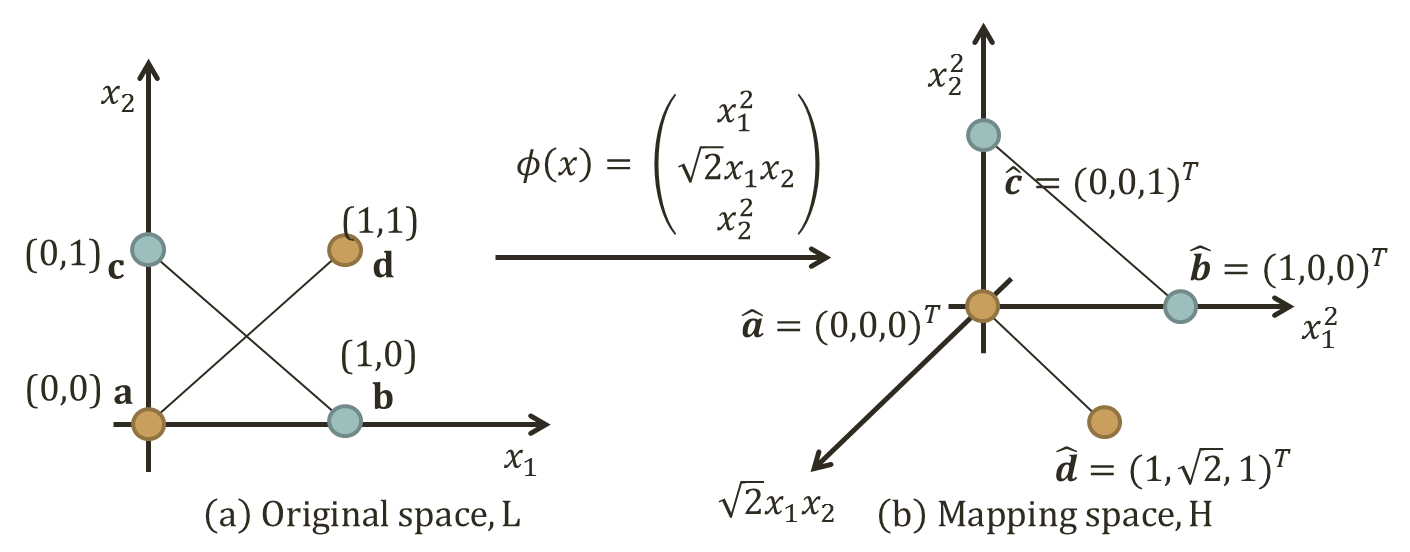
\includegraphics[scale=0.5]{Mapping}\caption{SVM 차원의 변환}\label{Fig:5-22}
\end{figure}\\
\indent 위의 그림 22에서 보면 기존 공간 L 에서는 선형 결정 경계로는 하늘색 점과 갈색 점이 분리할 수 없었지만 $\phi(x)$라는 mapping 함수를 통해 Basis를 확장하며 새로운 mapping 공간 H로 변환할 시 선형으로 분리가 가능하다. 하지만 이러한 확장 방법은, 위와 같이 작은 데이터셋에 대해서는 쉽게 이루어질 수 있지만, 데이터의 수가 매우 많아질 경우에는 Mapping 공간의 Basis가 걷잡을 수 없이 커질수가 있다는 문제점이 있다. 그래서 Mapping function을 어떻게 하면 이런 문제점을 해결할 수 있을 지 고민한 것에서부터 Kernel fuction의 아이디어가 나오게 되었다.

% 슬라이드 26
\indent 먼저 Kernel이란 기존과 다른 공간에서 두 벡터의 내적 값을 뜻한다. 수식으로 나타내면 다음과 같다.
\begin{equation}
K(x_i,x_j)=\varphi(x_i)\cdot\varphi(x_j)
\label{eq:5-33}
\end{equation}
즉, $x_i$와 $x_j$가 L 이라는 기존의 공간에 있었다면 $\phi$ 함수를 이용해 H라는 다른 공간 보낸 뒤, H 공간에서의 벡터 값끼리의 내적을 Kernel이라고 하는 것이다. 이러한 방법으로 다양한 종류의 Kernel 함수를 정의할 수 있다. 다음은 몇 가지 예시들을 나타내보았다.
\begin{itemize}\setlength\itemsep{-\parsep}
	\item 다항식(homogeneous)
	\begin{equation}
	k(x_i,x_j)=(x_i\cdot x_j)^d
	\label{eq:5-34}
	\end{equation}
\end{itemize}
\begin{itemize}\setlength\itemsep{-\parsep}
	\item 다항식(inhomogeneous)
	\begin{equation}
	k(x_i,x_j)=(x_i\cdot x_j+1)^d
	\label{eq:5-35}
	\end{equation}
\end{itemize}
\begin{itemize}\setlength\itemsep{-\parsep}
	\item Gaussian kernel function, a.k.a. Radial Basis Function
	\begin{equation}
	\begin{split}
	&k(x_i,x_j)={\exp}(-\gamma{\lVert x_i-x_j\rVert}^2)\\
	&For\ \gamma>0,\ Sometimes\ parameterize\ using\ \gamma=\frac{1}{2\sigma^2}
	\end{split}
	\label{eq:5-36}
	\end{equation}
\end{itemize}
\begin{itemize}\setlength\itemsep{-\parsep}
	\item Hyperbolic tangent, a.k.a. Sigmond Function
	\begin{equation}
	\begin{split}
	&k(x_i,x_j)={\tanh}(\kappa x_i\cdot x_j+c)\\
	&For\ some(not\ every)\ \kappa>0\ and\ c<0
	\end{split}
	\label{eq:5-37}
	\end{equation}
\end{itemize}

% 슬라이드 27
\indent 이들 중 한 가지 다항식 커널 함수에 대해서 예제를 보면서 살펴보도록 하겠다. 먼저 $\mathbf{x}=<x_1,x_2>$와 $\mathbf{z}=<z_1,z_2>$라고 두 개의 점이 있다고 생각해보자. 그리고 차원을 변화시키지 않은 차수 1의 다항식 커널 함수를 구하면 다음과 같다.
\begin{itemize}\setlength\itemsep{-\parsep}
	\item 차수 1의 다항식 커널 함수
\end{itemize}
\begin{equation}
K(<x_1,x_2>,<z_1,z_2>)=<x_1,x_2>\cdot<z_1,z_2>=x_1z_1+x_2z_2=\mathbf{x\cdot z}
\label{eq:5-38}
\end{equation}
다음으로는 차수 2의 다항식 커널 함수를 구해보겠다. 차수가 2로 늘어나면서 Basis를 3개로 확장하면, $\mathbf{x,z}$는 각각 3차원 공간의 점 $\phi(\mathbf{x})$와 $\phi(\mathbf{z})$으로 변환을 시킬 수 있다. 그리고 변환된 점에서의 내적을 구하고 식을 전개하면 다음과 같이 식이 정리가 된다.
\begin{itemize}\setlength\itemsep{-\parsep}
	\item 차수 2의 다항식 커널 함수
\end{itemize}
\begin{equation}
\begin{split}
&K(<x_1,x_2>,<z_1,z_2>)=<x_1^2,\sqrt{2}x_1x_2,x_2^2>\cdot<z_1^2,\sqrt{2}z_1z_2,z_2^2>\\
&=x_1^2 z_1^2+2x_1 x_2z_1z_2+x_2^2z_2^2=(x_1z_1+x_2z_2)^2=(\mathbf{x\cdot z})^2
\end{split}
\label{eq:5-39}
\end{equation}
위의 결과를 보면 $(\mathbf{x\cdot z})^2$의 결과를 띄는 것을 알 수 있다. 그리고 차수 3의 다항식 커널 함수에 대해서도 위와 같이 Basis를 확장해서 Kernel 값을 구하게 되면 다음과 같은 결과를 얻을 수 있다.
\begin{itemize}\setlength\itemsep{-\parsep}
	\item 차수 3의 다항식 커널 함수
\end{itemize}
\begin{equation}
K(<x_1,x_2>,<z_1,z_2>)=(\mathbf{x\cdot z})^3
\label{eq:5-40}
\end{equation}
이런식으로 차수 n의 다항식 커널 함수를 구해볼 수 있고, 모두 다음과 같은 형태를 갖게 된다.
\begin{itemize}\setlength\itemsep{-\parsep}
	\item 차수 n의 다항식 커널 함수
\end{itemize}
\begin{equation}
K(<x_1,x_2>,<z_1,z_2>)=(\mathbf{x\cdot z})^n
\label{eq:5-41}
\end{equation}
\indent 위의 결과가 의미하는 것을 살펴보도록 하겠다. 원래 커널 함수라고 하는 것은 기존의 두 점을 다른 차원의 공간으로 보내고 보내진 공간에서의 벡터(점)간의 내적이었는데, 기존의 두 점을 기존 공간에서 내적을 하고 다항식의 차수만큼 제곱을 해도 같은 값이 나온다는 것이다. 이는 커널 함수의 특징으로 굳이 다른 높은 차원으로 보낸 뒤 내적을 할 필요가 없다는 말이 된다. 즉, 커널 값을 알기 위해 힘들게 x와 z에 대해 변환된 좌표를 표현하고 계산할 필요가 없다는 것이다. 또한 높은 차수에서 선형 분리를 이용하기 위해서 공간을 변환할 필요도 없게 된다. 예를 들어 100 차원에서의 커널 값을 구하기 위해서 좌표를 100차원으로 변환하고 내적할 필요가 없이 기존 차원에서의 내적을 구한 뒤 이를 100제곱 하면 되는 것이다. 하지만 이 트릭으로 오직 내적만 계산이 가능하다는 조건이 있다.\\

% 슬라이드 28
\subsection{SVM with Kernel}
\indent 이제 Kernel 트릭을 Dual SVM에 적용을 해보도록 하겠다. 앞서서 우리가 선형으로 분리 가능하도록 만들기 위해 사용했던 방법들은 차원을 높이는 것이였다. 그래서 차원을 높이기 위해 Dual SVM의 목적함수를 다음과 같이 바꿔보겠다.
\begin{equation}
max_{\alpha\geq 0} \Sigma_j \alpha_j -\frac{1}{2}\Sigma_i \Sigma_j \alpha_i \alpha_j y_i y_j \varphi(x_i)\varphi(x_j)
\label{eq:5-42}
\end{equation}
그런데 여기에서 $\varphi$ 의 값을 굳이 구할 필요가 없다. 왜냐하면 $\varphi(x_i)\varphi(x_j)$ 부분은 Kernel 함수를 대체하면 되기 때문이다. 즉, 위의 목적 함수와 조건식은 다음과 같이 바꿀 수 있다.
\begin{equation}
\begin{split}
&max_{\alpha\geq 0} \Sigma_j \alpha_j -\frac{1}{2}\Sigma_i \Sigma_j \alpha_i \alpha_j y_i y_j K(x_i,x_j)\\
&s.t.\ \alpha_i ((wx_j+b)y_j-1)=0,C>\alpha_i>0\\
&\ \ \ \ \ \Sigma_{i=1}^{N} \alpha_i y_i =0\\
&\ \ \ \ \ C>\alpha_i>0,\forall i
\end{split}
\label{eq:5-43}
\end{equation}
이렇게 대체하게 되면 $x_i,x_j$값은 정해져서 알고 있기 때문에, Kernel 값 역시 미리 계산이 가능하다. 즉, 상수값처럼 다룰 수 있는 것이다. 또한 Kernel 함수는 다양한 종류가 있기 때문에 원하는 Kernel 함수를 다양하게 넣어볼 수 있다는 장점도 있다. 그리고 목적 함수를 수식 \eqref{eq:5-43}로 바꾸면 KKT 조건에 의해서 $\mathbf{w}$와 $b$는 다음과 같이 바뀌게 된다.
\begin{align}
&\mathbf{w}=\Sigma_{i=1}^{N} \alpha_i y_i \varphi(x_i)\label{eq:5-44}\\
&b=y_i-\Sigma_{i=1}^{N} \alpha_i y_i \varphi(x_i)\varphi(x_j)\label{eq:5-45}
\end{align}
그리고 b의 $\varphi(x_i)\varphi(x_j)$ 부분은 Kernel 값으로 대체가 가능하다. 그리고 $\mathbf{w}$에는 아직 $\varphi(x_i)$가 남아 있지만 이 역시 Kernel 값으로 대체가 가능한데 이는 바로 다음에서 유도를 해보도록 하겠다. 그리고 이와 같이 Kernel trick을 사용한 Dual 문제로 바꾸면 추정해야할 매개변수의 수를 줄일 수 있다. 또한 $\mathbf{w}$ 대신 $\alpha$ 값만 저장해도 된다.\\\\

% 슬라이드 29
\indent 이제 $\mathbf{w}$의 처리 방법에 대해서 알아보도록 하겠다. 수식 \eqref{eq:5-44}에서 보면 결정 경계의 방향성인 $\mathbf{w}$에 대해서는 여전히 $\varphi(x_i)$가 남아 있었다. 즉, $\mathbf{w}$를 알기 위해서는 차원을 mapping 해야한다는 것이다. 여기서 우리는 $\mathbf{w}$와 $b$를 구하는 이유에 대해서 다시 생각해볼 필요가 있다. 우리는 이 값들을 통해 f(x) 값을 구하여 Positive인지 Negative인지 Classification 하기 위해서 구하는 것이다. 즉, 우리는 결정 경계를 그리려고 하는 것이 목적이 아니라 결정 경계를 이용하여 임의의 인스턴스를 분류하는 것이 목적인 것이다. 따라서 $\mathbf{w}$값을 정확히 구할 필요가 없이 분류 값만 잘 구하면 되는 것이다.
\begin{figure}[ht]\centering
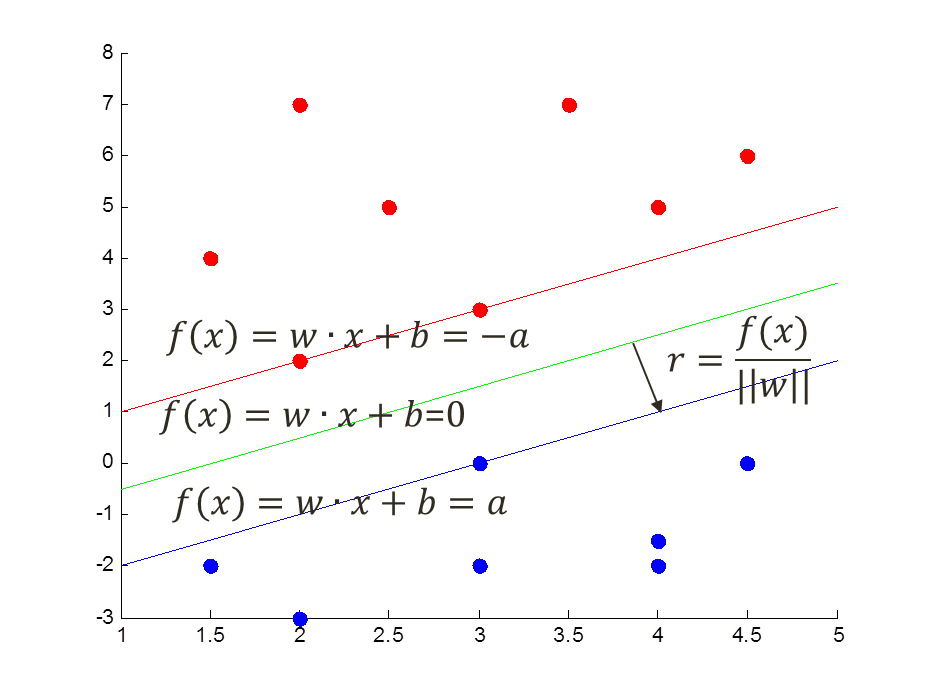
\includegraphics[scale=0.5]{SVM_kerneltrick}\caption{SVM의 분류}\label{Fig:5-23}
\end{figure}\\
\indent 먼저 SVM에 사용한 케이스에 따라 f(x)값의 부호와 최적화 식을 정리하면 다음과 같다.
\begin{itemize}\setlength\itemsep{-\parsep}
\item Linear case
\subitem $sign(w\cdot x+b)$
\subitem $min_{w,b} {\lVert w\rVert}$
\subitem $\ s.t.\ (wx_j+b)y_j\geq 1, \forall j$
\end{itemize}
\begin{itemize}\setlength\itemsep{-\parsep}
\item Transformed case
\subitem $sign(w\cdot\varphi(x)+b)$
\subitem $min_{w,b,\xi_j} {\lVert w\rVert}+C\Sigma_j \xi_j$
\subitem $\ s.t.\ (w\varphi(x_j)+b)y_j\geq1-\xi_j,\ \forall j$
\subitem $\ \ \ \ \ \ \xi_j\geq0,\ \forall j$
\end{itemize}
\begin{itemize}\setlength\itemsep{-\parsep}
\item Kernel trick case
\subitem $sign(w\cdot\varphi(x)+b)$
\subitem $max_{\alpha\geq 0} \Sigma_j \alpha_j- \frac{1}{2}\Sigma_i \Sigma_j \alpha_i \alpha_j y_i y_j K(x_i,x_j)$
\subitem $\ s.t.\ w=\Sigma_{i=1}^N\alpha_i y_i\varphi(x_i)$
\subitem $\ \ \ \ \ \ b=y_j-w\varphi(x_j)\ when\ 0<\alpha_j<C$
\subitem $\ \ \ \ \ \ \Sigma_{i=1}^{N} \alpha_i y_i=0$
\subitem $\ \ \ \ \ \ 0\leq \alpha_i\leq C,\forall i$
\end{itemize}
우리가 알아보고자 하는 것은 Kernel trick을 사용했을때 이므로, 마지막 케이스에 대해 살펴보고자 한다. $f(\varphi(x))$의 부호 값인 $sign(w\cdot\varphi(x)+b)$는 다른 조건식을 이용해 다음과 같이 전개 될 수 있다. 
\begin{equation}
\begin{split}
sign(w\cdot\varphi(x)+b)&=sign(\sum_{i=1}^N \alpha_i y_i \varphi(x_i)\cdot\varphi(x)+y_j-\sum_{i=1}^N \alpha_i y_i \varphi(x_i)\varphi(x_j))\\
&=sign(\sum_{i=1}^N \alpha_i y_i K(x_i,x)+y_j-\sum_{i=1}^N \alpha_i y_i K(x_i,x_j)),\ 0<\alpha_j<C
\end{split}
\label{eq:5-46}
\end{equation}
\indent 우리는 2차 계획법(quadratic programming)으로 $\alpha$를 얻을 수 있고, 데이터셋으로 $y$값을 이미 알고 있고, 커널값도 구할 수 있으므로 특정 x 에 대해서 분류 결과 값의 부호를 알 수 있다. 그리고 이 값의 결과가 양수이면 Positive로 분류하는 것이고 음수면 Negative로 분류를 하게 되는 것이다. 즉, 전처럼 w에 대한 해석과 w 값을 찾아내고, w를 이용해서 결정 경계선을 그리는 것은 불가능하나 Classification(분류)는 여전히 가능하다.\\

% 슬라이드 30
\begin{figure}[ht]\centering
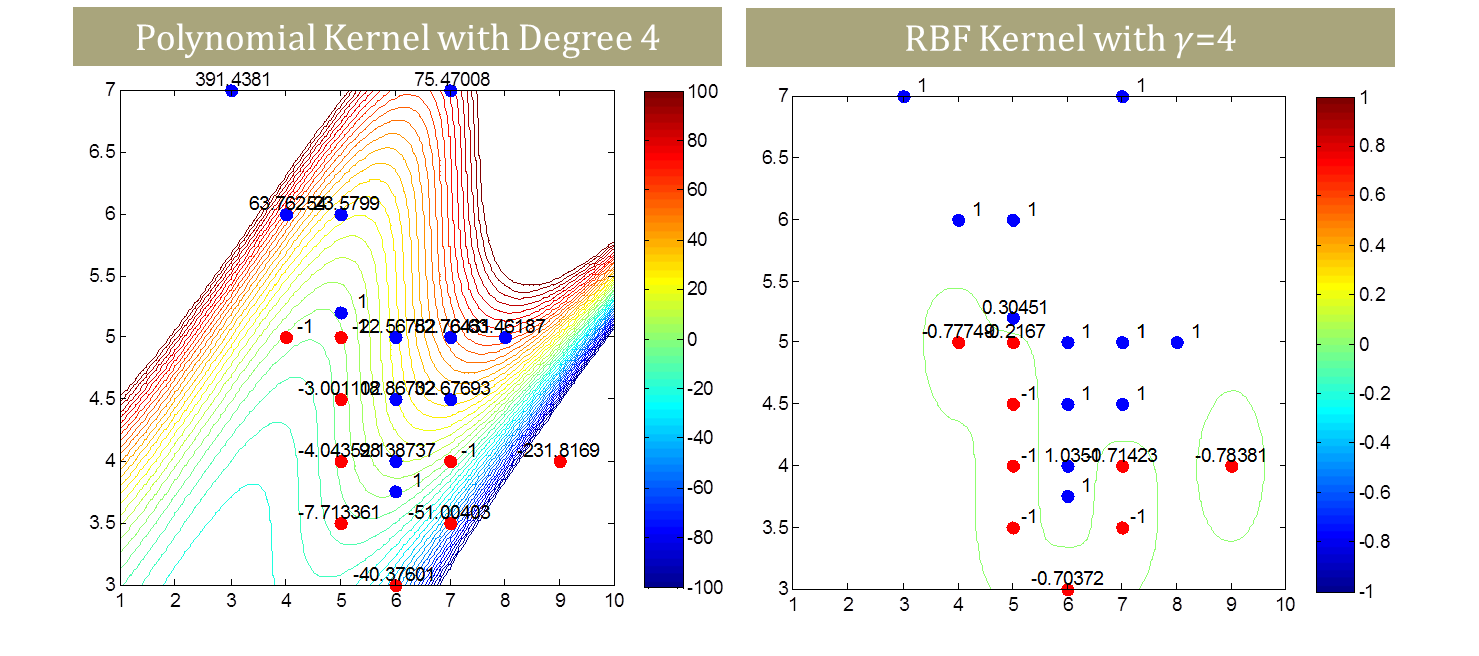
\includegraphics[scale=0.5]{SVM_variouskernel}\caption{다양한 Kernel을 이용한 SVM}\label{Fig:5-24}
\end{figure}
\indent Kernel trick을 이용한 SVM은 비선형으로 분리 가능한 경우에 대해 매우 적합하다. 그리고 고차원으로 쉽게 확장이 가능하다. 이를 바탕으로 다양한 Kernel 함수를 이용할 수 있다. 위 그림의 왼쪽 그림은 4 차수의 다항식 커널 함수를 이용해 SVM을 돌린 결과이고 오른쪽 그림은 RBF(Radial Basis Function) 커널 함수를 이용하여 SVM을 돌린 결과이다. 오른쪽 그림의 경우 결정 경계의 모양이 동그란 형태로 나오는 것을 확인할 수 있다.

% 슬라이드 31
\indent 로지스틱 회귀분석에도 커널을 사용할 수 있다. 로지스틱 회귀분석의 식은 $P(Y|X)=\frac{1}{1+e^{-\dot{\theta}T_x}}$였고 $\theta$의 MLE를 찾는 것이 목적이다. 여기서 $w=\Sigma_{i=1}^{N} \alpha_i y_i \varphi(x_i)$를 이용하여 $P(Y|X)$를 바꾸면 다음과 같이 된다.
\begin{equation}
P(Y|X)=\frac{1}{1+e^{-\dot{\theta}T_x}}=\frac{1}{1+e^{\Sigma_{i=1}^N \alpha_i y_i \varphi(x_i)\varphi(x)+b}}=\frac{1}{1+e^{\Sigma_{i=1}^N \alpha_i y_i \kappa(x_i,x)+b}}
\label{eq:5-47}
\end{equation}
이제 문제는 $\theta$를 찾는 것에서 $\alpha_i$를 찾는 것으로 바뀌었다. 이 문제를 해결하는 방법은 무엇일까? 다른 말로 제한된 최적화 문제인 것일까? 만약 그렇지 않다면 이것은 무엇을 의미하는 것일까? 한번 생각해보길 바란다.\\\\

\indent 여기까지 Kernel을 이용해서 복잡한 문제를 해결하는 방법에 대해서 배워보았다. 이번 장에서 배운 내용을 간략히 정리해보도록 하겠다. 먼저 서포트 벡터 머신이 Hard margin을 쓸 경우 현실의 데이터에 대해서 잘 동작하지 않았는데 에러 케이스에 대해 불가능한 해라고 판단을 했기 때문이었다. 이를 보완하기 위해서 Soft margin을 사용하여 페널티를 주는 방식을 생각했다. 하지만 이는 실제 데이터가 비선형으로 분리 가능한 경우에 대해서는 적용이 어려웠다. 그래서 높은 차원으로 데이터를 변환을 해야했는데 Kernel trick을 이용하면 이를 쉽게 할 수 있었다는 것이다. 그리고 이를 바탕으로 비선형의 데이터셋에 대해서도 Classification(분류)를 할 수 있게 되었다. 다음 장에서는 이러한 알고리즘으로 만든 모델이 잘 작동하는지 확인을 하는 방법에 대해서 배우도록 하겠다.

% 슬라이드 32
\section*{Acknowledgement}
\noindent This slideset is greatly influenced by
\begin{itemize}\setlength\itemsep{-\parsep}
\item Professor Carlos Guestrin at CMU
\item Professor Eric Xing at CMU
\end{itemize}

% 슬라이드 33
\section*{Further Readings}
\begin{itemize}
\setlength\itemsep{-\parsep}
\item Bishop Chapter 7 $\rightarrow$ 6
\end{itemize}

\end{document}
\end{document}
\end{document}